\documentclass[11pt, oneside]{article}
\usepackage{geometry} 
\geometry{letterpaper}
\usepackage{graphicx}	
\usepackage{amssymb, amsmath}
\usepackage{subfigure}
\usepackage{tikz}
\usepackage[colorlinks,citecolor=blue,urlcolor=blue]{hyperref}

\usetikzlibrary{intersections, backgrounds, calc}

\definecolor{light}{RGB}{220, 188, 188}
\definecolor{mid}{RGB}{185, 124, 124}
\definecolor{dark}{RGB}{143, 39, 39}
\definecolor{highlight}{RGB}{0, 255, 0}
\definecolor{gray60}{gray}{0.6}
\definecolor{gray70}{gray}{0.7}
\definecolor{gray80}{gray}{0.8}
\definecolor{gray90}{gray}{0.9}
\definecolor{gray95}{gray}{0.95}

\newcommand{\dd}{ \mathrm{d} }
\newcommand{\DD}{ \mathcal{D} }
\newcommand{\PP}{ \mathbb{P} }
\newcommand{\EE}{ \mathbb{E} }
\newcommand{\RR}{ \mathbb{R} }
\newcommand{\EV}[1]{\ensuremath { \mathcal{E} \! \left( #1 \right)  } }
\newcommand{\bt}{ \mbox{\boldmath{$\theta$}} }

\graphicspath{{figures/}}

\begin{document}

Uncertainty is inherent to learning and decision making, and it becomes all 
the more important when we try to formalize these processes.  For example,
measurement, the means of collecting the data from which we wish to learn, 
is fundamentally variable, and this variability must propagate to our inferences 
and any decisions based on them.  Consequently any formal technique for 
learning and decision making must be able to quantify uncertainty in a
self-consistent manner.  \emph{Bayesian inference} uses probability theory 
to quantify all forms of uncertainty, including not only the variability in 
measurements but also ignorance in the learning process itself.  

Because probability theory is so subtle and counterintuitive, introductory 
treatments of Bayesian inference often oversimplify and neglect many 
of the finer technical aspects.  Unfortunately, these technicalities have
a strong influence on practical applications of the theory, and without at 
least a conceptual understanding we are subject to dangerous fallacies.
In this review we attempt a deeper introduction to probability theory and 
Bayesian inference than usual to provide Stan users with the background 
necessary to properly wield Bayesian inference and take full advantage
of their measurements.

After reviewing some mathematical administration we'll introduce 
probability theory, keeping the presentation abstract but focusing on 
concepts instead of mathematical pedantry.  We'll then introduce how
we implement these abstract ideas in practice, both in terms of
concrete representations and computation, before discussing many
popular computational methods.  Finally we'll show how all of these
ideas come together in Bayesian inference.

\section{Mathematical Background and Notation}

Unfortunately, a thorough review of probability theory requires a nontrivial
mathematical background.  Although we strive to avoid as much mathematical
minutiae as possible, we have to assume that the reader is comfortable 
with the basics of differential and integral calculus over the real numbers.  
We highly encourage anyone who's math might be rusty to brush up before
proceeding.

We also assume familiarity with common set theory notation.  If $A$ is a set
then any element of the set is written as $a \in A$ while a subset is written
as $S \subset A$.  Sets are also sometimes denoted by their elements, for
example $A = \left\{ a_{1}, \ldots, a_{N} \right\}$.  The \emph{set builder
notation} is similarly used to denote subsets as 
$S = \left\{ a \in A \mid \cdot \right\}$, where $\cdot$ is the condition identifying
which elements of $A$ are in the subset $S \subset A$.  For example, we
can define the positive real numbers as 
%
\begin{equation*}
\RR^{+} = \left\{ x \in \RR \mid x > 0 \right\}.
\end{equation*}
%
The \emph{union} of two sets, $A \cup B$ is the combination of all 
elements in either set while the \emph{intersection} of two sets, 
$A \cap B$ is only those elements contained in both sets.

\emph{Spaces} are sets endowed with a structure called a 
\emph{topology} that allows us to separate ``well-behaved subsets''
from ``pathological subsets''.  We will assume that all of our sets
have such a structure and consequently for all intents and purposes 
set and space will be used interchangeably.  The only important
consequence of topologies that will be relevant for us is that ultimately
it is this topological structure that allows us to characterize spaces as 
either discrete or continuous.

Throughout we will use the common notation for maps from one set into 
another, $f : A \rightarrow B$ which defines $f$ as a map taking elements 
of the set $A$ to elements of the set $B$. In other words, $f(a) \in B$ for 
any $a \in A$.  Sometimes we will be more explicit regarding the action
on a given point and write
%
\begin{align*}
f &: A \rightarrow B \\
  &\quad a \mapsto f \! \left( a \right).
\end{align*}

When discussing computation we will liberally use $\approx$ to define
when two objects are approximately equal, or when we assume that
they are approximately equal, without making any effort to formally define
what ``approximately equal'' means.

\section{Probability in Theory}

Probability theory, and the measure theory on which it is based, is
a very detailed and intricate mathematical construction.  Here we will
make no attempt at the full mathematical rigor necessary for a complete
understanding, and instead focus on a high-level, conceptual intuition.  
This means, for example, that in many places we will appeal to vague 
notions like ``well-behaved'', as their technical definitions do not offer
much pedagogical benefit.

The fundamental objects in probability theory are probability distributions
defined over event spaces.  In this section these objects are defined
only abstractly, which unfortunately means that we cannot rely on
helpful visualizations to support the definitions and manipulations.
To use a probability distribution in any practical application, including
visualization, we need some means of specifying and utilizing them 
explicitly, which will have to wait until the next section.

\subsection{Logical Statements and Events}

\emph{Logical statements} are the general way to specify information 
about a system.  For example, if $\bt$ is an object that takes values 
in the space $\Theta$ then we can make statements like $\bt = \theta$ 
or $\theta_{1} < \bt < \theta_{2}$.

One potential use of logical statements is to describe the outcome
of a variable measurement, or an event.  Indeed this is exactly the 
application on which modern probability theory was based and,
unfortunately, this also means that the terminology in probability 
theory focuses on this particular application instead of more general 
logical statements.  In order to avoid conflicting with standard 
terminology, going forward we will refer to logical statements as 
events, but it is important to keep in mind the more general interpretation.

More formally, consider quantifying information about an object $\bt$
which takes values in the space $\Theta$.  $\Theta$ is known as the 
\emph{sample space}, and it allows us to explicitly specify logical 
statements about $\bt$.  Logical statements, or \emph{events}, $E$, 
as specified by well-behaved subset of the sample space, 
$E \subset \Theta$.  We also denote the \emph{event space} of 
well-behaved subsets of the sample space as $\EV{\Theta}$.

For example, if $\bt$ took values on the real line, $\Theta = \RR$, then 
events could be points in the sample space, $E = \left\{ \theta = 5 \right\}$, 
intervals, $E = \left\{ \theta \in \Theta \mid \theta < 5 \right\}$ or 
$E = \left\{ \theta \in \Theta \mid 1 < \theta < 5 \right\}$, or various
combinations of the two, such as
%
\begin{equation*}
E = 
\left\{ \theta = -5 \right\}
\cup
\left\{ \theta \in \Theta \mid 1 < \theta < 5 \right\}
\cup
\left\{ \theta \in \Theta \mid 10 < \theta < 12 \right\}.
\end{equation*}
%
Event spaces always include the null event, $E = \emptyset$, and the 
trivial event, $E = \Theta$.

One subtlety with this construction is that we can specify the
same logical statements, and hence events, using different 
sample spaces.  Consider, for example, an invertible map 
from one sample space into another, $s : \Theta \rightarrow \Omega$.  
If every event in $\Theta$ maps to an event in $\Omega$
and vice versa,
%
\begin{align*}
s \! \left( E_{\Theta} \right) &\in \EV{\Omega}
\\
s^{-1} \! \left( E_{\Omega} \right) &\in \EV{\Theta}
\end{align*}
%
then the map is called \emph{measurable} and the two
sample spaces can be used to specify the same logical 
statements.  When a measurable map exists between
two sample spaces we say that they are \emph{equivalent}
as they provide equivalent descriptions of the same system.

In other words, there are many ways to describe any given system,
and hence different ways to explicitly specify logical statements.
These different specifications, however, all quantify the same 
information.

\subsection{Probability Distributions}

If we are uncertain about our target system, $\bt$, then we cannot
ensure that any particular event is true.  Instead all we can do
is quantify our uncertainty about $\bt$ by assigning each event a
\emph{probability} that quantifies which events are more likely to
be true than others.  Probabilities themselves are bounded between 
0, indicating that an event is absolutely false, and 1, indicating that 
an event is absolutely true.

In probability theory probabilities are assigned to events by a \emph{probability 
distribution},
%
\begin{equation*}
\PP : \mathcal{E} \! \left( \Theta \right) \rightarrow \left[0, 1 \right],
\end{equation*}
%
where $\left[0, 1\right]$ is the interval
%
\begin{equation*}
\left[ 0, 1 \right] = \left\{ x \in \RR \mid 0 \le x \le 1 \right\}.
\end{equation*}
%
The probability of the null event is zero, 
$\PP \! \left[ \emptyset \right] = 0$, and the probability of the trivial
event is one, $\PP \! \left[ \Theta \right] = 1$.  These latter
two conditions are an immediate consequence of our initial
assumption that $\bt$ has to take values in the sample space.

If logical statements quantify information about the system $\bt$, 
then probability distributions quantify our uncertainty about those 
statements and hence our uncertainty about the the system itself.  
When using a probability distribution to 
quantify our uncertainty about $\bt$ we often write $\bt \sim \PP$ which 
is usually read as, ``$\bt$ is distributed according to the probability 
distribution $\PP$'' but should really read ``Logical statements about 
$\bt$ are distributed according to the probability distribution $\PP$''.

These probability assignments satisfy the usual rules of probability, 
such as the sum rule,
%
\begin{equation*}
\PP \! \left[ E_{1} \cup E_{2} \right]
= 
\PP \! \left[ E_{1} \right] + \PP \! \left[ E_{2} \right] 
- \PP \! \left[ E_{1} \cap E_{2} \right],
\end{equation*}
%
and the exclusion rule,
%
\begin{equation*}
\PP \! \left[ E \right] 
= 
\PP \! \left[ \Theta \right] - \PP \! \left[ E^{c} \right]
=
1 - \PP \! \left[ E^{c} \right],
\end{equation*}
%
where $E^{c}$ is the \emph{complement} of $E$ satisfying
$E \cup E^{c} = \Theta$.

Probability distributions also allow us to compute \emph{expectation values} 
of well-behaved functions on the sample space,
%
\begin{equation*}
\EE_{\PP} : \mathcal{F} \! \left( \Theta \right) \rightarrow \mathbb{R},
\end{equation*}
%
where $\mathcal{F} \! \left( \Theta \right)$ is the collection of well-behaved 
functions $f : \Theta \rightarrow \mathbb{R}$.  Common expectations 
include means, variances, and higher-order moments.  In fact, we
can also consider probability assignments themselves as expectations,
%
\begin{equation*}
\PP \! \left[ E \right] = \EE_{\PP} \! \left[ \mathbb{I}_{E} \right],
\end{equation*}
%
where the \emph{indicator function} of the event $E$, $\mathbb{I}_{E}$,
is defined as
%
\begin{equation*}
\mathbb{I}_{E} \! \left( \theta \right)
= 
\left\{
\begin{array}{rr}
0, & \theta \notin E \\
1, & \theta \in E
\end{array}
\right. .
\end{equation*}

The most important consequence of these definitions is that \emph{all of 
probability theory reduces to computing expectations}.  Any other operation 
that you may have encountered in probability theory can only ever be an
intermediate step in computing a final expectation.  In particular, many of 
the more non-intuitive aspects of probability theory can avoided by carefully
framing everything as an expectation -- don't try to intuit solutions, calculate 
them!

\subsection{Conditional Probability Distributions}

Reasoning about probability distributions on low-dimensional spaces
is usually straightforward -- or at least as straightforward as the
mathematics will allow -- but reasoning about probability distributions
on high-dimensional spaces is much more subtle.  One
very elegant way to simplify these high-dimensional probability
distributions is to treat them as a product of simpler, one-dimensional
probability distributions know as \emph{conditional probability
distributions}.

A conditional probability distribution is a set of probability distributions 
indexed by some auxiliary space, $\Phi$,
%
\begin{align*}
\PP_{\Theta \mid \Phi} 
&: \EV{\Theta} \times \Phi \rightarrow \left[0, 1 \right] \\
&\quad \left( E_{\Theta}, \phi \right) \;\; \mapsto 
\PP_{\Theta \mid \Phi} \! \left[ E_{\Theta} \mid \phi \right].
\end{align*}
%
In other words, for any value of $\phi \in \Phi$ the conditional probability
distribution defines a probability distribution on $\Theta$, and for any
event in $\Theta$ the conditional probability distribution defines a 
function from $\Phi$ to probabilities.  By combining a conditional
probability distribution with a probability distribution on the conditioning
space, $\Phi$, we can construct a probability distribution on the joint
sample space, $\Theta \times \Phi$.

This \emph{joint distribution} is defined implicitly by its probability assignments
or expectation values.  For example, the probability of any joint event, 
$E_{\Theta} \times E_{\Phi}$, is given by first using the conditional 
probability distribution to assign a probability to $E_{\Theta}$, 
$\PP_{\Theta|\Phi} \! \left[ E_{\Theta} \mid \phi \right]$, and then 
taking the expectation of this assignment over the distribution on $\Phi$,
%
\begin{equation*}
\PP_{\Theta \times \Phi} \! \left[ E_{\Theta} \times E_{\Phi} \right]
=
\mathbb{E}_{\PP_{\Phi}} \! \left[  
\PP_{\Theta|\Phi} \! \left[ E_{\Theta} \mid \phi \right] 
\cdot \mathbb{I}_{E_{\Phi}} \! \left( \phi \right)
\right],
\end{equation*}
%
where the indicator function, $\mathbb{I}_{E_{\Phi}}$, ensures that we 
take the expectation only over the event in $\Phi$.  Similarly, joint 
expectations are defined iteratively as
%
\begin{equation*}
\EE_{\PP_{\Theta \times \Phi}} \! \left[ g \! \left( \theta, \phi \right) \right]
=
\mathbb{E}_{\PP_{\Phi}} \! \left[  
\EE_{\PP_{\Theta|\Phi}} \! \Big[ 
g \! \left( \theta, \phi \right) \mid \phi 
\Big]
\right].
\end{equation*}

If we consider only the trivial event on the conditioning space $E_{\Phi} 
= \Phi$, then this construction also defines a  \emph{marginal distribution} 
on $\Theta$ by
%
\begin{align*}
\PP_{\Theta} \! \left[ E_{\Theta} \right]
&\equiv
\PP_{\Theta \times \Phi} \! \left[ E_{\Theta} \times \Phi \right] \\
&=
\mathbb{E}_{\PP_{\Phi}} \! \left[  
\PP_{\Theta|\Phi} \! \left[ E_{\Theta} \mid \phi \right]
\right],
\end{align*}
or
%
\begin{align*}
\EE_{\PP_{\Theta}} \! \left[ f \! \left( \theta \right) \right]
&\equiv
\EE_{\PP_{\Theta \times \Phi}} \! \left[ f \! \left( \theta \right) \right] \\
&=
\mathbb{E}_{\PP_{\Phi}} \! \left[  
\EE_{\PP_{\Theta|\Phi}} \! \Big[ 
f \! \left( \theta \right) \mid \phi 
\Big]
\right].
\end{align*}
%
This marginalization process allows us to collapse a joint probability 
distribution onto any of the component spaces while taking into account 
all correlations between the components.

Consequently, conditional probability distributions are powerful ways of
building probability distributions on high-dimensional spaces.  We simply 
start with a probability distribution on one low-dimensional component and 
then build up a joint distribution using conditional probability distributions 
for each new component,
%
\begin{align*}
& \PP_{\Theta_{1}} \\
& \PP_{\Theta_{2} \mid \Theta_{1}} \\
& \PP_{\Theta_{3} \mid \Theta_{2}, \Theta_{1}} \\
& \cdots \\
& \PP_{\Theta_{N} \mid \Theta_{N - 1}, \ldots, \Theta_{2}, \Theta_{1}}.
\end{align*}
%
These conditional probability distributions are often naturally motivated by
the problem at hand and, if we think about deterministic processes as 
degenerate conditional probability distributions that assign all probability 
to a single event for each conditioning value,
%
\begin{equation*}
\PP_{\Theta \mid \Phi} \! \left[ E_{\Theta} \mid \phi \right]
= 
\left\{
\begin{array}{rr}
0, & E_{\Theta} \ne \hat{E} \! \left( \phi \right) \\
1, & E_{\Theta} = \hat{E} \! \left( \phi \right)
\end{array}
\right.,
\end{equation*}
%
then these conditional probability distributions can also incorporate 
deterministic and even causal relationships.  This iterative process 
of building a joint probability distribution from conditional probability 
distributions is known as \emph{generative modeling}.

\subsection{The Invariance of Probability Distributions}

Like events, probability distributions can be defined with respect
to many different sample spaces.  If $s : \Theta \rightarrow 
\Omega$ is a measurable map and $\PP_{\Theta}$ is a probability
distribution defined over events in $\Theta$, then we can define an 
equivalent probability distribution over events in $\Omega$ by 
assigning probabilities as
%
\begin{equation*}
\PP_{\Omega} \! \left[ E_{\Omega} \right]
\equiv
\PP_{\Theta} \! \left[ s^{-1} \! \left( E_{\Omega} \right) \right].
\end{equation*}
%
Furthermore, this whole process can be inverted: if $\PP_{\Omega}$ 
is a probability distribution defined over events in $\Omega$ then 
we can define an equivalent probability distribution over events in 
$\Theta$ by assigning probabilities as
%
\begin{equation*}
\PP_{\Theta} \! \left[ E_{\Theta} \right]
\equiv
\PP_{\Omega} \! \left[ s \! \left( E_{\Theta} \right) \right].
\end{equation*}

Just like events, probability distributions are invariant when we
move between equivalent sample spaces.  Different but equivalent
sample spaces are just different ways to describe the same system,
with events quantifying the same, invariant information and probability 
distributions quantifying the same, invariant uncertainty.

\section{Probability in Practice: Specifying Distributions}

As we saw in the previous section, abstract notions of probability
distributions are not particularly easy to intuit, and abstract
probability distributions are not easily specified or manipulated
in practical applications.  When the sample space is structured, 
however, that structure can be leveraged to provide the explicit 
specifications we need to apply probability theory in practice.  
This is particularly evident when the sample space is discrete 
or a subset of the real numbers.

\subsection{Representations of Probability Distributions over
Discrete Sample Spaces}

When the sample space is discrete we can completely specify a
probability distribution by assigning probability to only a small
and manageable set of events.  Two particularly convenient sets,
point events and interval events, allow us to represent probability
distributions with probability mass functions and cumulative 
distribution functions, respectively.  

\subsubsection{Probability Mass Functions}

\emph{Probability mass functions} assign probably to point events,
those events that are simply elements of the original sample space.  
Hence a probability mass function is a just function that assigns a 
probability to each element of the sample space,
%
\begin{equation*}
p : \Theta \rightarrow \left[0, 1\right].
\end{equation*}

In this case more general event probabilities are given by simply summing 
the probability of each element in event,
%
\begin{equation*}
\PP \! \left[ E \right]
=
\sum_{\theta \in E} p \! \left( \theta \right).
\end{equation*}
%
Similarly, expectations are given by summing the probability of each 
element of the sample space, weighted by the function value,
%
\begin{equation*}
\mathbb{E} \! \left[ f \right]
=
\sum_{\theta \in \Theta} f \! \left( \theta \right) p \! \left( \theta \right),
\end{equation*}
%
for any $f \in \mathcal{F} \! \left( \Theta \right)$.

Probability mass functions also have the convenient property that
they are invariant to the particular choice of sample space.  Given
a measurable map $s : \Theta \rightarrow \Omega$ and a probability 
mass function on $\Theta$, we can define an equivalent probability 
mass function on $\Omega$ as
%
\begin{equation*}
p_{\Omega} \! \left( \omega \right) 
\equiv 
p_{\Theta} \! \left( s^{-1} \! \left( \omega \right) \right).
\end{equation*}

\subsubsection{Conditional Probability Mass Functions}

Probability mass functions can be extended to represent conditional probability
distributions by simply adding a conditioning variable,
%
\begin{equation*}
p_{\Theta \mid \Phi} : \Theta \times \Phi \rightarrow \left[0, 1\right],
\end{equation*}
%
with conditional probabilities and conditional expectations computed
as above,
%
\begin{align*}
\PP_{\Theta \mid \Phi}  \! \left[ E \mid \phi \right]
&=
\sum_{\theta \in E} p_{\Theta \mid \Phi}  \! \left( \theta \mid \phi \right),
\\
\mathbb{E}_{\PP_{\Theta \mid \Phi} } \! \left[ f \mid \phi \right]
&=
\sum_{\theta \in \Theta} f \! \left( \theta \right) 
p_{\Theta \mid \Phi}  \! \left( \theta \mid \phi \right),
\end{align*}

A huge advantage of this representation is that it drastically simplifies the
construction of joint and marginal probability distributions.  Instead of implicitly
defining an abstract joint distribution, for example, we can compute an 
explicit joint probability mass function,
%
\begin{equation*}
p_{\Theta \times \Phi} \! \left( \theta, \phi \right) = 
p_{\Theta \mid \Phi} \! \left( \theta | \phi \right) p_{\Phi} \! \left( \phi \right),
\end{equation*}
%
which readily gives joint probabilities and joint expectations.

Marginalization proceeds similarly -- the marginal probability mass function
is given by simply summing the joint probability mass function over the
nuisance components,
%
\begin{align*}
p_{\Theta} \! \left( \theta \right)
&= 
\sum_{\phi \in \Phi}  p_{\Theta \times \Phi} \! \left( \theta, \phi \right) \\
&=
\sum_{\phi \in \Phi}
p_{\Theta \mid \Phi} \! \left( \theta | \phi \right) p_{\Phi} \! \left( \phi \right).
\end{align*}

\subsubsection{Cumulative Distribution Functions}

When the sample space is not only discrete but also ordered then we
can also completely specify a probability distribution by assigning
probabilities to \emph{intervals}, 
$\mathcal{I} \! \left( \Theta \right) \subset \mathcal{E} \! \left( \Theta \right)$.
Intervals are events spanning all points less than or equal to some 
distinguished point, $\theta$,
%
\begin{equation*}
I \! \left( \theta \right) = \left\{ \theta' \in \Theta \mid \theta' \leq \theta \right\}.
\end{equation*}
%
The function that assigns these probabilities,
%
\begin{align*}
P 
&: \Theta \rightarrow \mathcal{I} \! 
\left( \Theta \right) \rightarrow \left[0, 1 \right]
\\
&\quad \theta \mapsto 
I \! \left( \theta \right) \;\; \mapsto 
\PP \! \left[ I \! \left( \theta \right) \right].
\end{align*}
%
is called the \emph{cumulative distribution function}.  

As with the probability mass function, cumulative distributions functions
immediately map between sample spaces.  For a measureable map
$s : \Theta \rightarrow \Omega$ we have
%
\begin{equation*}
P_{\Omega} \! \left( I_{\omega} \right) 
\equiv 
P_{\Theta} \! \left( s^{-1} \! \left( I_{\omega} \right) \right).
\end{equation*}

\subsubsection{Relating Probability Mass Functions and Cumulative 
Distribution Functions}

Because probability mass functions and cumulative distribution functions both
specify the same probability distribution, one can always be used to construct
the other.  Given a probability mass function, for example, we can construct
the cumulative distribution function as
%
\begin{equation*}
P \! \left( \theta \right)
= \PP \! \left[ I \! \left( \theta \right) \right]
= \sum_{\theta' \in I ( \theta )} p \! \left( \theta' \right).
\end{equation*}
%
Similarly, we can construct a probability mass function from a cumulative
distribution function as
%
\begin{equation*}
p \! \left( \theta \right) = 
P \! \left( \theta \right)
- P \! \left( \theta_{-} \right),
\end{equation*}
%
where $\theta_{-}$ is the largest element of $\Theta$ less that $\theta$,
%
\begin{equation*}
\theta_{-} = \max \left\{ \theta' \in \Theta \mid \theta' < \theta \right\}.
\end{equation*}

\subsection{Representations of Probability Distributions over the Real
Numbers}

When the sample space is the $D$-dimensional real numbers, or
a subset thereof, there is an uncountably infinite number of point events.  
Not only can we no longer assign a non-zero probability to each point 
event without having most event probabilities explode, $\PP \! \left[ E \right]
\rightarrow \infty$, we can't even define the sums over the sample space 
necessary to compute probabilities and expectations!  

Instead of assigning to each point a probability we have to assign  
to each point event a \emph{probability density}  which we can 
\emph{integrate} to give probabilities and expectations.  Assigning 
probabilities to intervals, however, is still sufficient so we can also 
define cumulative distribution functions on these spaces.

\subsubsection{Probability Density Functions}

A \emph{probability density function} assigns a positive value to each
point in the sample space
%
\begin{equation*}
p : \Theta \rightarrow \mathbb{R}^{+}.
\end{equation*}
%
These values, known as \emph{probability densities}, have no particular 
meaning of their own and instead exist only to be integrated to give 
probabilities,
%
\begin{equation*}
\PP \! \left[ E \right]
=
\int_{E} p \! \left( \theta \right) \dd \theta,
\end{equation*}
%
and expectations,
%
\begin{equation*}
\mathbb{E} \! \left[ f \right]
=
\int_{\Theta} f \! \left( \theta \right) p \! \left( \theta \right) \dd \theta.
\end{equation*}

This is an important point that is worth repeating -- probability densities 
are meaningless until they have been integrated over some event.  To 
analogize with physics, the event over which we integrate corresponds 
to a \emph{volume} and the probability given by integrating the density 
over such a volume corresponds to a \emph{mass}.  When we want to 
be careful to differentiate between probabilities and probability densities 
we'll use \emph{probability mass} to refer to the former.

One of the most awkward properties of these representations is that, 
unlike probability mass functions, probability density functions do not
readily transform between sample spaces.  Specifically, for the
measurable map $s : \Theta \rightarrow \Omega$
%
\begin{equation*}
p_{\Omega} \! \left( \omega \right)
\neq
p_{\Theta} \! \left( s^{-1} \! \left( \omega \right) \right)!
\end{equation*}

The problem with the real numbers is that mapping between sample
spaces transforms not only the event space but also how we differentiate
and integrate.  Under a well-behaved map $s : \Theta \rightarrow \Omega$ 
the corresponding differential volumes are related by
%
\begin{equation*}
\dd \omega = \left| \mathbf{J} \right| \dd \theta,
\end{equation*}
%
where the matrix
%
\begin{equation*}
J_{ij} 
= 
\frac{\partial \omega_{i} }{ \partial \theta_{j} }
\equiv 
\frac{ \partial s_{i} }{ \partial \theta_{j} }
\end{equation*} 
%
is called the \emph{Jacobian} of the transformation.  Consequently
all integrals are invariant to the particular sample space if and only
if the probability density functions are related by
%
\begin{equation*}
p_{\Omega} \! \left( \omega \right) 
= 
p_{\Theta} \! \left( s^{-1} \! \left( \omega \right) \right) | \mathbf{J} |^{-1}.
\end{equation*}
%
Each sample space has its own differential volume and probability density 
function but \emph{the same integrals} and, hence, the same probabilities 
and expectations (Figure \ref{fig:pdf_transform}).  This dependence on the
sample space is another reason to be careful not to take a probability
density function in isolation too seriously.

\begin{figure*}
\centering
%
\subfigure[]{
%\begin{tikzpicture}[scale=0.3, thick, show background rectangle]
\begin{tikzpicture}[scale=0.3, thick]
  \node[] at (0,0) {\includegraphics[width=5cm]{density.eps}};
  \foreach \i in {-10.5, -10, ..., 10.5} {
    \draw[-, color=gray80] (-11, \i) to (11, \i);
    \draw[-, color=gray80] (\i, -11) to (\i, 11);
  }  
  \node[] at (0,0) {\includegraphics[width=5cm]{area.eps}};
  \node[] at (0, -13) { $\PP \! \left[ E_{\Theta} \right] = \int_{E_{\Theta}} 
                                   p_{\Theta} (\theta_{1}, \theta_{2}) 
                                   \dd \theta_{1} \dd \theta_{2} $ };
\end{tikzpicture}
}
%
\subfigure[]{
%\begin{tikzpicture}[scale=0.3, thick, show background rectangle]
\begin{tikzpicture}[scale=0.3, thick]
  \node[] at (0,0) {\includegraphics[width=5cm]{transformed_density.eps}};
  \foreach \i in {-10.9969, -10.9428, -10.8857, -10.8251, -10.7605, -10.6915, -10.6174, 
                        -10.5374, -10.4504, -10.355, -10.2497, -10.1319, -9.99835, -9.84419, 
                        -9.66186, -9.4387, -9.15099, -8.74547, -8.05217, 0., 8.05217, 
                        8.74547, 9.15099, 9.4387, 9.66186, 9.84419, 9.99835, 10.1319, 
                        10.2497, 10.355, 10.4504, 10.5374, 10.6174, 10.6915, 10.7605,
                        10.8251, 10.8857, 10.9428, 10.9969} {
    \draw[-, color=gray80] (-11, \i) to (11, \i);
    \draw[-, color=gray80] (\i, -11) to (\i, 11);
  }  
  \node[] at (0,0) {\includegraphics[width=5cm]{transformed_area.eps}};
  \node[] at (0, -13) { $\PP \! \left[ s \! \left( E_{\Theta} \right) \right] 
                                   = \int_{s(E_{\Theta})} 
                                   p_{\Omega} (\omega_{1}, \omega_{2}) 
                                   \dd \omega_{1} \dd \omega_{2}$ };
\end{tikzpicture}
}
\caption{When sample spaces are real, each sample space has
its own density functions (red), events (green), and differential volumes 
(grey).  Here the sample space in (b) is related to the sample space in 
(a) by the compatible mapping $\left(\omega_{1}, \omega_{2} \right) 
= s \!\left( \theta_{1}, \theta_{2} \right)$. All of these differences, however, 
exactly compensate to ensure that integrals always yield the same 
values, here $\PP \! \left[ E_{\Theta} \right]  = 
\PP \! \left[ s \! \left( E_{\Theta} \right) \right] $.
}
\label{fig:pdf_transform}
\end{figure*}

A helpful mnemonic for the arrangement of the Jacobian in these 
transformations is to remember that the integrand must be invariant,
%
\begin{align*}
p_{\Omega} \! \left( \omega \right) \dd \omega
&=
p_{\Theta} \! \left( \theta \right) \dd \theta
\\
p_{\Omega} \! \left( \theta \right)
&= 
p_{\Theta} \! \left( \theta \right) \frac{ \dd \theta }{ \dd \omega }
\\
p_{\Omega} \! \left( \omega \right)
&= 
p_{\Theta} \! \left( \theta \right) \left| \mathbf{J} \right|^{-1}.
\end{align*}

For a concrete example, consider a two-dimensional sample space 
with real components $\left( \theta_{1}, \theta_{2} \right)$ and a 
probability distribution represented with a Gaussian probability density,
%
\begin{equation*}
p_{\Theta} \! \left( \theta_{1}, \theta_{2} \right)
\propto
\exp \! \left( - \frac{\theta_{1}^{2} + \theta_{2}^{2}}{2} \right).
\end{equation*}
%
We can then introduce a second sample space with the map
%
\begin{equation*}
\left( \omega_{1}, \omega_{2} \right) 
= 
r \! \left( \theta_{1}, \theta_{2} \right) 
= 
\left( s \! \left( \theta_{1} \right), s \! \left( \theta_{2} \right) \right),
\end{equation*}
%
where the component maps are given by
%
\begin{equation*}
s \! \left( \theta \right)
=
\log \! \left(
\frac{ \pi + 2 \, \mathrm{atan} \! \left( \alpha \, \theta \right) }
{ \pi - 2 \, \mathrm{atan} \! \left( \alpha \, \theta \right) }
\right)
\end{equation*}
%
with the inverse
%
\begin{equation*}
s^{-1} \! \left( \omega \right)
=
\frac{1}{\alpha} 
\tan \! \left(
\frac{\pi}{2} \, \frac{e^{\omega} - 1}{e^{\omega} + 1} \right)
\end{equation*}
%
and Jacobian
%
\begin{equation*}
J \! \left( \omega \right)
=
\frac{ \partial s }{ \partial \theta } \! \left( \omega \right)
=
\frac{\alpha}{\pi} \frac{ \left( 1 + e^{\omega} \right)^{2} }{ e^{\omega} }
\sin^{2} \! \left( \frac{ \pi }{ 1 + e^{\omega} } \right).
\end{equation*}
%
The Jacobian of the complete map is then given by
%
\begin{equation*}
\mathbf{J} = 
\begin{bmatrix}
J & 0 \\
0 & J
\end{bmatrix},
\end{equation*}
%
with the determinant $| \mathbf{J} | = J^{2}$.  Hence the transformed
probability density function and differential volume are given by
%
\begin{equation*}
p_{\Omega} \! \left( \omega_{1}, \omega_{2} \right)
=
p_{\Theta} \! \left( 
s^{-1} \! \left( \omega_{1} \right), 
s^{-1} \! \left( \omega_{2} \right) \right)
J^{-2} \! \left( \omega \right)
\end{equation*}
%
and
%
\begin{equation*}
\dd \omega_{1} \dd \omega_{2}
=
J^{2} \dd \theta_{1} \dd \theta_{2},
\end{equation*}
%
respectively.  These two realizations are shown graphically in 
(Figure \ref{fig:pdf_transform}).

\subsubsection{Conditional Probability Density Functions}

Just as in the discrete case, probability density functions can be immediately
extended to represent conditional probability distributions by simply adding a 
conditioning variable,
%
\begin{equation*}
p_{\Theta \mid \Phi} : \Theta \times \Phi \rightarrow \mathbb{R}^{+},
\end{equation*}
%
with conditional probabilities and conditional expectations computed
as integrals,
%
\begin{align*}
\PP_{\Theta \mid \Phi}  \! \left[ E \mid \phi \right]
&=
\int_{E} p_{\Theta \mid \Phi}  \! \left( \theta \mid \phi \right) \dd \theta,
\\
\mathbb{E}_{\PP_{\Theta \mid \Phi} } \! \left[ f \mid \phi \right]
&=
\int_{\Theta} f \! \left( \theta \right) 
p_{\Theta \mid \Phi}  \! \left( \theta \mid \phi \right) \dd \theta,
\end{align*}

Likewise, probability density functions representing joint and marginal 
probability distributions are easy to construct for conditional probability 
density functions.  Joint probability density functions are given by a simple
multiplication,
%
\begin{equation*}
p_{\Theta \times \Phi} \! \left( \theta, \phi \right) = 
p_{\Theta \mid \Phi} \! \left( \theta | \phi \right) p_{\Phi} \! \left( \phi \right),
\end{equation*}
%
and marginal probability density functions are given by integrating out the
nuisance components,
%
\begin{align*}
p_{\Theta} \! \left( \theta \right)
&= 
\int_{\Phi} p_{\Theta \times \Phi} \! \left( \theta, \phi \right) \dd \phi \\
&=
\int_{\Phi}
p_{\Theta \mid \Phi} \! \left( \theta | \phi \right) 
p_{\Phi} \! \left( \phi \right) \dd \phi.
\end{align*}

\subsubsection{Cumulative Distribution Functions}

Because the real numbers are sufficiently well-ordered, we can also 
specify probability distributions over these spaces by assigning probability 
to intervals using a cumulative distribution function,
%
\begin{align*}
P 
&: \Theta \rightarrow \mathcal{I} \! \left( \Theta \right) 
\rightarrow 
\left[0, 1 \right]
\\
&\quad \theta 
\mapsto 
I \! \left( \theta \right) \;\; 
\mapsto 
\PP \! \left[ I \! \left( \theta \right) \right].
\end{align*}
%
where each interval, $I \! \left( \theta \right) \in \mathcal{I} \! 
\left( \Theta \right)$, is defined as before,
%
\begin{equation*}
I \! \left( \theta \right) = \left\{ \theta' \in \Theta \mid \theta' \leq \theta \right\}.
\end{equation*}

Unlike probability density functions, and similar to discrete cumulative
distribution functions, real cumulative distributions functions
immediately map between sample spaces,
%
\begin{equation*}
P_{\Omega} \! \left( I_{\omega} \right) 
\equiv 
P_{\Theta} \! \left( s^{-1} \! \left( I_{\omega} \right) \right)
\end{equation*}
%
for a measurable map $s : \Theta \rightarrow \Omega$.

\subsubsection{Relating Probability Mass Functions and Cumulative 
Distribution Functions}

On the real numbers probability density functions and cumulative 
distribution functions are also equivalent and can be mapped into 
each other.  Cumulative distribution functions, for example, are given 
by integrating over probability density functions,
%
\begin{equation*}
P \! \left( \theta \right)
= \PP \! \left[ I \! \left( \theta \right) \right]
= \int_{\theta_{\min}}^{\theta} p \! \left( \theta' \right) \dd \theta.
\end{equation*}

Probability density functions, on the other hand, are given by 
differentiating cumulative distribution functions,
%
\begin{equation*}
p \! \left( \theta \right) = 
\frac{\partial P \! \left( \theta \right) }{ \partial \theta}.
\end{equation*}
%
Note that if we map to an equivalent sample space, 
$s : \Theta \rightarrow \Omega$, then the derivative
acquires a factor of the inverse Jacobian so that the
corresponding probability density function transforms
as necessary,
%
\begin{equation*}
p \! \left( \omega \right) 
= 
\frac{\partial P \! \left( \omega \right) }{ \partial \omega}
=
\frac{\partial P \! \left( s^{-1} \! \left( \omega \right) \right) }
{ \partial \theta}
\frac{ \partial \theta }{ \partial \omega }
= 
p \! \left( s^{-1} \! \left( \omega \right) \right) \left| J^{-1} \right|.
\end{equation*}

\subsection{Representations of Mixed Probability Distributions}

Distributions over samples spaces that have both a discrete, $\Phi$,
and a real $\Psi$, component can be specified by leveraging 
discrete and continuous representations of conditional distributions.  

For example, a distribution over $\Theta = \Phi \times \Psi$ can be
specified by conditioning the discrete component with the real
component, $\PP_{\Phi \mid \Psi}$, and providing a marginal distribution
over the real component, $\PP_{\Psi}$.  Using a conditional
probability mass function for the former and a probability density function
for the latter, the probability of any event is given by
%
\begin{align*}
\PP_{\Theta} \! \left[ E \right]
&=
\PP_{\Theta} \! \left[ E_{\Phi} \times E_{\Psi} \right]
\\
&=
\EE_{\PP_{\Psi}} \! \left[
\PP_{\Phi \mid \Psi} \! \left[  E_{\Phi} \mid \psi \right]
\cdot
\mathbb{I}_{E_{\Psi}} \! \left( \psi \right)
\right] 
\\
&= 
\int_{E_{\Psi} }
\sum_{\phi \in E_{\Phi} } p_{\Phi \mid \Psi} \! \left( \phi \mid \psi \right)
p_{\Psi} \! \left( \psi \right) \dd \psi,
\end{align*}
%
with expectations given similarly by
%
\begin{align*}
\EE_{\PP_{\Theta}} \! \left[ f \right]
&=
\EE_{\PP_{\Psi}} \! \left[
\EE_{\PP_{\Phi \mid \Psi}} \! \left[  f \mid \psi \right]
\right] 
\\
&= 
\int_{E_{\Psi} } \sum_{\phi \in E_{\Phi} } f \! \left( \phi, \psi \right) 
p_{\Phi \mid \Psi} \! \left( \phi \mid \psi \right)
p_{\Psi} \! \left( \psi \right) \dd \psi.
\end{align*}

Equivalently, we could also condition the real component on the
discrete component, $\PP_{\Psi \mid \Phi}$, and provide a marginal 
distribution over the discrete component, $\PP_{\Phi}$.  We could 
then represent the distribution with a conditional probability density 
function for the former and a probability mass function for the latter.  
Likewise, the probability of any event is given by
%
\begin{align*}
\PP_{\Theta} \! \left[ E \right]
&=
\PP_{\Theta} \! \left[ E_{\Phi} \times E_{\Psi} \right]
\\
&=
\EE_{\PP_{\Phi}} \! \left[
\PP_{\Psi \mid \Phi} \! \left[  E_{\Psi} \mid \phi \right]
\cdot
\mathbb{I}_{E_{\Phi}} \! \left( \phi \right)
\right] 
\\
&= 
\sum_{\phi \in E_{\Phi} } \int_{E_{\Psi} }
p_{\Psi \mid \Phi} \! \left( \psi \mid \phi \right) 
p_{\Phi} \! \left( \phi \right) \dd \psi,
\end{align*}
%
with expectations given similarly by
%
\begin{align*}
\EE_{\PP_{\Theta}} \! \left[ f \right]
&=
\EE_{\PP_{\Phi}} \! \left[
\EE_{\PP_{\Psi \mid \Phi}} \! \left[  f \mid \phi \right]
\right] 
\\
&= 
\sum_{\phi \in E_{\Phi} } \int_{E_{\Psi} }
f \! \left( \phi, \psi \right) 
p_{\Psi \mid \Phi} \! \left( \psi \mid \phi \right)
p_{\Phi} \! \left( \phi \right) \dd \psi.
\end{align*}

Regardless of how we choose to decompose the mixed distribution,
combining probability density functions and probability mass functions
makes specifying and manipulating distributions straightforward in
practice.

\subsection{Stochastic Representations of Probability Distributions}

We can also represent any probability distribution, including both
discrete and real probability distributions, \emph{stochastically}.  
A \emph{stochastic process} is any mechanism that generates a 
sequence of states, or \emph{samples} from a given sample space, 
$\left\{ \theta_{1}, \ldots, \theta_{N} \right\} \subset \Theta$.  Such a 
mechanism is equivalent to a given probability distribution if the 
samples themselves can be used to recover all expectations as 
the size of the sequence becomes infinitely large. More formally, 
if
%
\begin{equation*}
\lim_{N \rightarrow \infty} \frac{1}{N} f \! \left( \theta_{n} \right)
= \EE_{\PP} \! \left[ f \right],
\end{equation*}
%
for all well-behaved functions, $f : \Theta \rightarrow \RR$, then the 
stochastic process is equivalent to the probability distribution $\PP$.

This procedure, and hence the resulting samples, are \emph{exact} 
if every element in the generated sequence is independent of every 
other element.  In other words, samples are exact when the stochastic
process generates samples one at a time, with no dependence on the 
preceding or following samples.  If samples are not exact we refer to
them as \emph{correlated}.

Exact stochastic processes are, by construction, perfectly
\emph{random} processes: there is no way to predict any element 
of the sampling sequence given the state of other samples in
that sequence.  Unfortunately such randomness is impossible to 
achieve in practice as computers are fundamentally deterministic.
Instead we rely on \emph{pseudorandom} processes which
generate sequences in a convoluted but ultimately deterministic
fashion.  When we are ignorant of the precise configuration of a
pseudorandom process the resulting samples are effectively
random

Pseudorandom processes that target specific probability distributions, 
or \emph{pseudorandom number generators}, can be devised for 
many simple probability distributions.  Unfortunately they are typically 
impossible to construct for the more complex distributions that are
often of practical interest.

\section{Probability in Practice: The Complexity of Computation}

The beauty of probability theory is that, once we have selected a
\emph{target} probability distribution, the only well-posed computations
are expectations.  As noted above, the many subtleties and apparent 
paradoxes of probability theory are readily overcome by ignoring our
typically-biased intuition and instead posing questions as expectations
and computing.

Once we've settled on a representation of our probability distribution, 
these computations reduce to straightforward manipulations, either 
summations in the discrete case or integration in the real case.  
Unfortunately, the conceptual elegance of these computations does not 
imply that the calculations themselves are trivial.  

Outside of the most simple problems the necessary summations and 
integrations cannot be calculated analytically and we must be satisfied 
with only approximate estimates.  Moreover, the only way to guarantee
accurate estimation is to exhaustively survey the sample space, and
for large sample spaces the cost of such surveys easily overwhelm our 
finite computational resources.  Consequently, computationally efficient 
yet accurate estimates requires more sophisticated approaches that take
advantage of the geometry of the target probability distribution itself.

In this section we study the geometry of probability distributions
on high-dimensional sample spaces and how that geometry frustrates
approximate algorithms, both in theory and with an explicit example.  
From here on we will consider only real sample spaces -- much of the 
intuition we will develop does carry over to the discrete case, but 
developing algorithms around that corresponding intuition is still an 
open problem in statistics.

\subsection{Concentration of Measure}

The key to constructing robust estimates of any expectation is identifying 
which neighborhoods of our target sample space contribute to the 
corresponding integrals; any computation outside of those relevant 
neighborhoods is wasted.  How to identify those relevant neighborhoods 
for a given target distribution, however, is not immediately obvious
All that we know is that, because those neighborhoods define expectations,
they should be equivalent for equivalent sample spaces.

Naively we might consider a neighborhood around the mode of our 
representative probability density function where the density, and 
presumably also contributions to any integral, is largest.  This
neighborhood, however, is dependent on the particular sample
space and hence doesn't have the necessary invariance properties.
Our intuition must be missing something important.

Indeed, our naive intuition overlooks the \emph{volume} over which 
we integrate the probability density functions.  Although probability 
density functions concentrate around their modes, the volume over which
we integrate does not.  As we move towards infinity there is more and
more room over which we can integrate, especially in high-dimensions.
Consequently the integrand, which is the \emph{product} of these two 
contributions, concentrates in a singular neighborhood somewhere in the 
middle known as the \emph{typical set} (Figure \ref{fig:typical_set}) in
a phenomenon is known as \emph{concentration of measure}

\begin{figure*}
\centering

\begin{tikzpicture}[scale=0.35, thick]

  \begin{scope}
    \clip (-12, -6) rectangle (12, 10);
    \foreach \i in {0, 0.05,..., 1} {
      \draw[line width={30 * \i}, opacity={exp(-8 * \i)}, dark] 
        (-10, 0) .. controls (-10, 15) and (-5, 5) .. (0, 5)
        .. controls (5, 5) and (10, 8) .. (10, 0)
        .. controls (10, -8) and (5, -3) .. (0, -3)
        .. controls (-5, -3) and (-10, -5) .. (-10, 0);
    }  
  \end{scope}
\end{tikzpicture}
\caption{On high-dimensional samples spaces all well-behaved probability 
distributions concentrate in a neighborhood called the \emph{typical set}.  
In order to estimate the integrals needed to compute probabilities and 
expectations we have to be able to identify where the typical set lies in 
the sample space which is no easy task.
}
\label{fig:typical_set}
\end{figure*}

Transformations between equivalent sample spaces may change where 
the probability density and volume concentrate, but these changes always 
cancel exactly to yield an equivalent typical set.  Concentration of measure 
and the typical set are properties of a probability distribution itself and not 
of any particular sample space we use to specify that distribution.

Although this analysis is too vague to help us identify the typical set
for a given probability distribution, it does provide crucial understanding 
of why high-dimensional expectations are so difficult to compute.  For 
example, because probability is distributed across the entire typical set, 
no \emph{single} point in the sample space yields a good approximation 
to all expectations:
%
\begin{quote}
\emph{to construct estimators that are accurate for many expectations 
we need to quantify the entire typical set.}
\end{quote}
%
Moreover, because points outside of the typical set contribute little to 
nothing to any integral,
%
\begin{quote}
\emph{we need to focus the entirely of our computational resources on 
evaluations within only the typical set.}
\end{quote}
%  
Finally, because the typical set is a property of a probability distribution 
itself,
%
\begin{quote}
\emph{all of our computational algorithms should be independent of the 
details of any particular representation,  such as the mode of a probability 
density function.}
\end{quote}

\subsection{An Explicit Example of Concentration of Measure}

Concentration of measure can be difficult to reconcile with our
low-dimensional intuition, so let's examine an explicit example.  Consider 
a probability distribution over the $D$-dimensional real numbers 
represented by a product of Gaussian probability density functions,
%
\begin{equation*}
p \! \left( \theta \right) = 
\prod_{d = 1}^{D} \frac{1}{\sqrt{2 \pi \sigma^{2} } }
\exp \! \left( - \frac{\theta_{d}^{2}}{2 \sigma^{2}} \right),
\end{equation*}
%
with the corresponding differential volume,
%
\begin{equation*}
\dd V = \prod_{d = 1}^{D} \dd \theta_{d}.
\end{equation*}
%
In order to identify which neighborhoods of the sample space contribute
most to generic expectations, we now transform to a sample space with 
spherical coordinates.  This yields the probability density function
%
\begin{equation*}
p \! \left( r, \phi_{1}, \ldots, \phi_{D - 1} \right) = 
\left( \frac{1}{2 \pi \sigma^{2} } \right)^{\frac{D}{2}}
\exp \! \left( - \frac{r^{2}}{2 \sigma^{2}} \right),
\end{equation*}
%
with the corresponding differential volume,
%
\begin{equation*}
\dd V = 
r^{D - 1} \dd r 
\prod_{d = 1}^{D - 1} \sin^{D - d - 1} \! \left( \phi_{d} \right) \dd \phi_{d}.
\end{equation*}
%
Because the probability density function does not depend on
any of the hyperspherical angles, neither will any probabilities
and, consequently, any neighborhood of high probability must be
spherically symmetric.  To see where these neighborhoods concentrate
radially we can marginalize out the hyperspherical angles analytically
to give the radial probability density function,
%
\begin{equation*}
p \! \left( r \right) = 
\left( 2 \sigma^{2} \right)^{-\frac{D}{2} }
\frac{ 2 }{ \Gamma \! \left( \frac{D}{2} \right) }
r^{D - 1} \exp \! \left( - \frac{r^{2}}{2 \sigma^{2}} \right),
\end{equation*}
%
which is exactly the scaled $\chi$ distribution.  In particular, for
large $D$ all of the probability concentrates in a neighborhood
around $r \approx \sigma \sqrt{D}$ with width around $\sigma / \sqrt{2}$.  
In other words, almost all of our target probability can be found in a 
thin shell at $r = \sigma \sqrt{D}$ and that neighborhood concentrates 
tighter and tighter around that shell as we add more and more dimensions 
(Figure \ref{fig:conc_of_meas_anal}).

\begin{figure*}
\centering
\includegraphics[width=3in]{conc_of_meas_anal.eps}
\caption{In high dimensions real probability distributions generically 
assign almost all of their probability into a singular neighborhood known as
the typical set.  This is apparent even from a probability density function 
representation: although the density concentrates around the corresponding
mode, the volume over which we integrate that density is much larger away
from the mode.  These two opposing trends balance to give the typical set.}
\label{fig:conc_of_meas_anal}
\end{figure*}

Because samples recover all expectations asymptotically, they have
must concentrate across the typical set (Figure \ref{fig:samples}).
Consequently, we can also use samples to simulate concentrate of 
measure.  For a given $D$ we can generate a sample from our target 
probability using a univariate Gaussian random number generator 
available in any computing library,
%
\begin{equation*}
\theta_{n} \sim \mathcal{N} \! \left(0, \sigma^{2} \right),
\end{equation*}
%
with the corresponding radial distance $r = \sqrt{ \sum_{d = 1}^{D} x_{d}^{2} }$.
Generating a sequence of samples and then histogramming the radial 
distance reveals the same $\chi$ distribution that we arrived at analytically
(Figure \ref{fig:concentration_of_measure_emp}).

\begin{figure*}
\centering
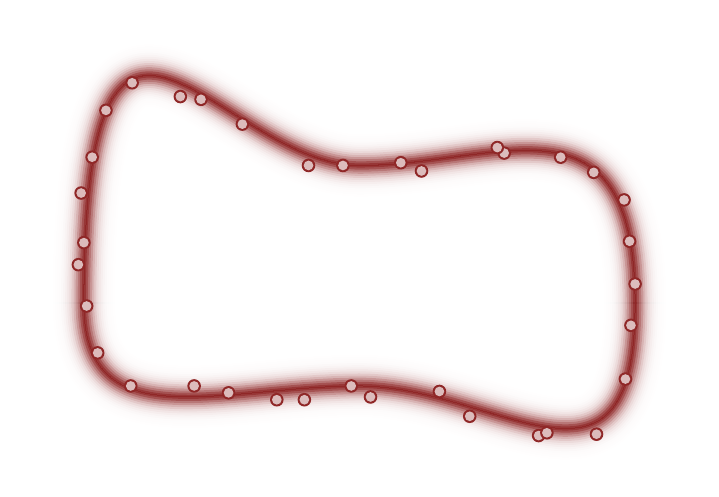
\begin{tikzpicture}[scale=0.35, thick]
  \draw[-,color=white] (-12, 0) to (12, 0);
  
  \begin{scope}
  \clip (-12, -6) rectangle (12, 10);
  \foreach \i in {0, 0.05,..., 1} {
    \draw[line width={30 * \i}, opacity={exp(-8 * \i)}, dark] 
      (-10, 0) .. controls (-10, 15) and (-5, 5) .. (0, 5)
      .. controls (5, 5) and (10, 8) .. (10, 0)
      .. controls (10, -8) and (5, -3) .. (0, -3)
      .. controls (-5, -3) and (-10, -5) .. (-10, 0);
  }
  
  % Mixing
  \fill[color=dark] (-6, -3) circle (7pt);  
  \fill[color=light] (-6, -3) circle (5pt);
  
  \fill[color=dark] (-4.75, -3.25) circle (7pt);  
  \fill[color=light] (-4.75, -3.25) circle (5pt);
  
  \fill[color=dark] (-3, -3.5) circle (7pt);  
  \fill[color=light] (-3, -3.5) circle (5pt);
  
  \fill[color=dark] (-2, -3.5) circle (7pt);  
  \fill[color=light] (-2, -3.5) circle (5pt);
  
  \fill[color=dark] (-0.3, -3) circle (7pt);  
  \fill[color=light] (-0.3, -3) circle (5pt);  
  
  \fill[color=dark] (0.4, -3.4) circle (7pt);  
  \fill[color=light] (0.4, -3.4) circle (5pt);
  
  \fill[color=dark] (2.9, -3.2) circle (7pt);  
  \fill[color=light] (2.9, -3.2) circle (5pt);
  
  \fill[color=dark] (4, -4.1) circle (7pt);  
  \fill[color=light] (4, -4.1) circle (5pt);
  
  \fill[color=dark] (6.5, -4.8) circle (7pt);  
  \fill[color=light] (6.5, -4.8) circle (5pt);
  
  \fill[color=dark] (6.8, -4.7) circle (7pt);  
  \fill[color=light] (6.8, -4.7) circle (5pt);
  
  \fill[color=dark] (8.6, -4.75) circle (7pt);  
  \fill[color=light] (8.6, -4.75) circle (5pt);
  
  \fill[color=dark] (9.65, -2.75) circle (7pt);  
  \fill[color=light] (9.65, -2.75) circle (5pt);
  
  \fill[color=dark] (9.85, -0.8) circle (7pt);  
  \fill[color=light] (9.85, -0.8) circle (5pt);
  
  \fill[color=dark] (10, 0.7) circle (7pt);  
  \fill[color=light] (10, 0.7) circle (5pt);
  
  \fill[color=dark] (9.8, 2.25) circle (7pt);  
  \fill[color=light] (9.8, 2.25) circle (5pt);
  
  \fill[color=dark] (9.6, 3.75) circle (7pt);  
  \fill[color=light] (9.6, 3.75) circle (5pt);
  
  \fill[color=dark] (8.5, 4.75) circle (7pt);  
  \fill[color=light] (8.5, 4.75) circle (5pt);

  \fill[color=dark] (7.3, 5.3) circle (7pt);  
  \fill[color=light] (7.3, 5.3) circle (5pt);
  
  \fill[color=dark] (5.25, 5.45) circle (7pt);  
  \fill[color=light] (5.25, 5.45) circle (5pt);
  
  \fill[color=dark] (5, 5.65) circle (7pt);  
  \fill[color=light] (5, 5.65) circle (5pt);
  
  \fill[color=dark] (2.25, 4.8) circle (7pt);  
  \fill[color=light] (2.25, 4.8) circle (5pt);
  
  \fill[color=dark] (1.5, 5.1) circle (7pt);  
  \fill[color=light] (1.5, 5.1) circle (5pt);
  
  \fill[color=dark] (-0.6, 5) circle (7pt);  
  \fill[color=light] (-0.6, 5) circle (5pt);
  
  \fill[color=dark] (-1.85, 5) circle (7pt);  
  \fill[color=light] (-1.85, 5) circle (5pt);
  
  \fill[color=dark] (-4.25, 6.5) circle (7pt);  
  \fill[color=light] (-4.25, 6.5) circle (5pt);

  \fill[color=dark] (-5.75, 7.4) circle (7pt);  
  \fill[color=light] (-5.75, 7.4) circle (5pt);
  
  \fill[color=dark] (-6.5, 7.5) circle (7pt);  
  \fill[color=light] (-6.5, 7.5) circle (5pt);
  
  \fill[color=dark] (-8.25, 8) circle (7pt);  
  \fill[color=light] (-8.25, 8) circle (5pt);
  
  \fill[color=dark] (-9.2, 7) circle (7pt);  
  \fill[color=light] (-9.2, 7) circle (5pt);
  
  \fill[color=dark] (-9.7, 5.3) circle (7pt);  
  \fill[color=light] (-9.7, 5.3) circle (5pt);
  
  \fill[color=dark] (-10.1, 4) circle (7pt);  
  \fill[color=light] (-10.1, 4) circle (5pt);
  
  \fill[color=dark] (-10, 2.2) circle (7pt);  
  \fill[color=light] (-10, 2.2) circle (5pt);  
  
  \fill[color=dark] (-10.2, 1.4) circle (7pt);  
  \fill[color=light] (-10.2, 1.4) circle (5pt);  

  \fill[color=dark] (-9.9, -0.1) circle (7pt);  
  \fill[color=light] (-9.9, -0.1) circle (5pt);  

  \fill[color=dark] (-9.5, -1.8) circle (7pt);  
  \fill[color=light] (-9.5, -1.8) circle (5pt);  

  \fill[color=dark] (-8.3, -3) circle (7pt);  
  \fill[color=light] (-8.3, -3) circle (5pt);  
  
  \end{scope}
\end{tikzpicture}
\caption{Because samples recover expectations asymptotically,
large sequences of samples must concentrate in the typical set.
This provides a means of visualizing concentration of measure,
and will prove a powerful way to estimate expectations.
}
\label{fig:samples}
\end{figure*}

\begin{figure*}
\centering
\subfigure[]{ \includegraphics[width=1.85in]{gauss_hist1.eps} }
\subfigure[]{ \includegraphics[width=1.85in]{gauss_hist2.eps} }
\subfigure[]{ \includegraphics[width=1.85in]{gauss_hist3.eps} }
\caption{Concentration of measure can be visualized with samples 
from a given distribution, which concentrate across the typical set.  
For low-dimensions the concentration is weak the the typical set 
is diffuse, but as the dimensionality of the target distribution grows
so do does the concentration of measure.
}
\label{fig:concentration_of_measure_emp}
\end{figure*}

\section{Probability in Practice: Deterministic Estimators}

If we can't quantify the target typical set exactly, one immediately
strategy is to just replace it with a simpler one.  In other words,
we can approximate a complex target distribution, $\PP$, with a 
simpler distribution, $\widetilde{\PP}$, whose expectations, or at 
least some expectations of practical interest, are known analytically,
%
\begin{equation*}
\EE_{\PP} \! \left[ f \right] 
\approx 
\EE_{\widetilde{\PP}} \! \left[ f \right].
\end{equation*}

\emph{Deterministic estimators} use various criteria to identify an 
optimal approximating distribution so that expectations can be 
approximated deterministically.

\subsection{MAP Estimators}

Ideally all expectations with respect to our approximating distribution 
would be analytic so that we could use it to approximate any 
expectation with respect to our target distribution.  The only
probability distribution that fits this criteria is the \emph{Dirac distribution},
$\mathbb{D}_{\tilde{\theta}}$, that assigns all probability to a single point 
in the sample space, $\tilde{\theta}$,
%
\begin{equation*}
\mathbb{D}_{\tilde{\theta}} \! \left[ E \right] = 
\left\{
\begin{array}{rr}
0, & \tilde{\theta} \notin E  \\
1, & \tilde{\theta} \in E
\end{array}
\right. .
\end{equation*}
%
Because all probability concentrates at $\tilde{\theta}$, expectations 
are trivial,
%
\begin{equation*}
\EE_{\mathbb{D}} \! \left[ f \right] 
=
 f \! \left( \tilde{\theta} \right).
\end{equation*} 

Where, however, should we assign all probability to best approximate
the target distribution and its typical set?  One of the simplest, and 
consequently most popular, deterministic estimation strategies is 
\emph{maximum a posteriori}, or \emph{MAP}, estimation.  In MAP
estimation we approximate the target distribution with a Dirac distribution 
at the mode of the probability density function,
%
\begin{equation*}
\theta_{\mathrm{MAP}} = \mathrm{argmax} \, p \! \left( \theta \right).
\end{equation*}


This approach, however, immediately contradicts the intuition provided by 
concentration of measure: it utilizes a single point in the sample space
that lies outside of the typical set and depends entirely on the choice of
probability density function representation!  Why, then, is MAP estimation
so ubiquitous?

MAP estimators are seductive because the optimization on which they
rely is relatively computationally inexpensive.  Moreover, in some very 
simple cases MAP estimators constructed from probability density function
in \emph{some} sample spaces can be reasonably accurate for 
\emph{some} functions.  For example, if the target probability distribution 
is sufficiently simple that the typical set is convex \emph{and} if a 
sample space can be found such that the mode of the probability density 
function lies in the center of that typical set, then the corresponding MAP 
estimator might yield reasonably accurate estimates for the mean, 
$\EE_{\PP_{\Theta}} \! \left[ \theta \right]$ (Figure \ref{fig:good_map_bad_map}).

\begin{figure*}
\centering
\subfigure[]{
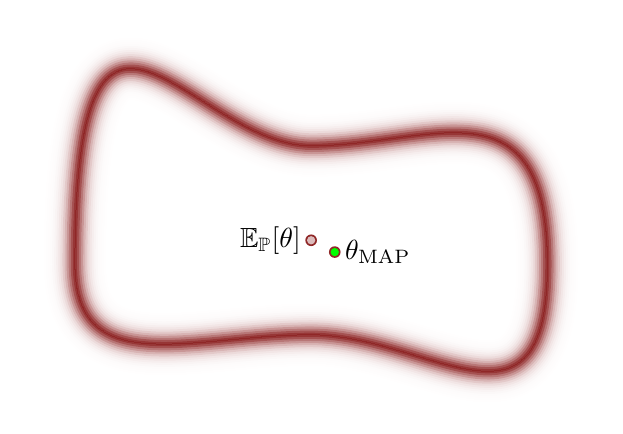
\begin{tikzpicture}[scale=0.3, thick]

  \begin{scope}
    \clip (-12, -6) rectangle (12, 10);
    \foreach \i in {0, 0.05,..., 1} {
      \draw[line width={30 * \i}, opacity={exp(-8 * \i)}, dark] 
        (-10, 0) .. controls (-10, 15) and (-5, 5) .. (0, 5)
        .. controls (5, 5) and (10, 8) .. (10, 0)
        .. controls (10, -8) and (5, -3) .. (0, -3)
        .. controls (-5, -3) and (-10, -5) .. (-10, 0);
    }  
  \end{scope}
  
  \fill[color=dark] (0, 1) circle (7pt);  
  \fill[color=light] (0, 1) circle (5pt)
  node[left, color=black]  { $\EE_{\PP} \! \left[ \theta \right]$ };
 
  \fill[color=dark] (1, 0.5) circle (7pt);
  \fill[color=green] (1, 0.5) circle (5pt)
  node[right, color=black]  { $\theta_{\mathrm{MAP}}$ };
  
\end{tikzpicture}
}
\subfigure[]{
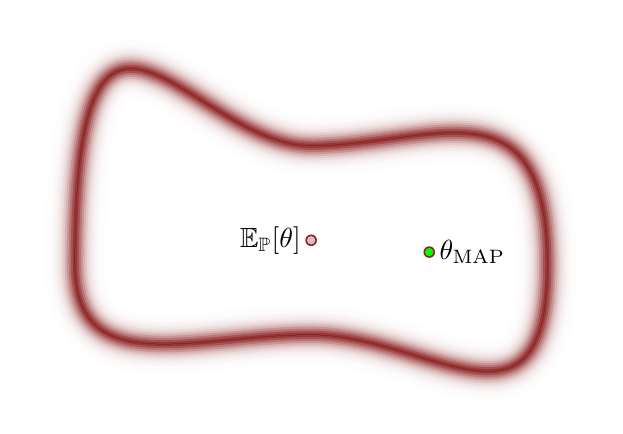
\begin{tikzpicture}[scale=0.3, thick]

  \begin{scope}
    \clip (-12, -6) rectangle (12, 10);
    \foreach \i in {0, 0.05,..., 1} {
      \draw[line width={30 * \i}, opacity={exp(-8 * \i)}, dark] 
        (-10, 0) .. controls (-10, 15) and (-5, 5) .. (0, 5)
        .. controls (5, 5) and (10, 8) .. (10, 0)
        .. controls (10, -8) and (5, -3) .. (0, -3)
        .. controls (-5, -3) and (-10, -5) .. (-10, 0);
    }  
  \end{scope}
  
  \fill[color=dark] (0, 1) circle (7pt);  
  \fill[color=light] (0, 1) circle (5pt)
  node[left, color=black]  { $\EE_{\PP} \! \left[ \theta \right]$ };
 
  \fill[color=dark] (5, 0.5) circle (7pt);
  \fill[color=green] (5, 0.5) circle (5pt)
  node[right, color=black]  { $\theta_{\mathrm{MAP}}$ };
  
\end{tikzpicture}
}
\caption{(a) In simple cases a prescient choice of sample space can 
yield a MAP estimator that well approximates some expectations, 
such as the mean of the real parameters $\theta$.  (b) Poor choices 
of the representation, however, yield very inaccurate estimates, even 
in these simple problems.
}
\label{fig:good_map_bad_map}
\end{figure*}

Because they rely on a point estimate, however, MAP estimators are 
terrible at approximating expectations that depend on the breadth of 
the typical set, such as the variance.  Furthermore, identifying the optimal 
sample space, even if one exists, for a particular target function is 
extremely challenging in practice.  Worse, we have no generic means
of even quantifying the error in these estimators for a generic target
distribution.  Ultimately this strong sensitivity to the choice of sample 
space and inability to validate the accuracy of the estimators makes MAP
estimation extremely fragile in practice.

\subsection{Laplace Estimators}

The fragility of MAP estimators can be partially resolved by generalizing
them to \emph{Laplace estimators} which approximate the probability
density function with a Gaussian density function,
%
\begin{equation*}
p \! \left( \theta \right) \approx 
\mathcal{N} \! \left( \theta \mid \mu, \Sigma \right),
\end{equation*}
%
where the mean is given by the MAP estimate,
%
\begin{equation*}
\mu = \theta_{\mathrm{MAP}},
\end{equation*}
%
and the covariance is given by the Hessian of the probability density 
function,
%
\begin{equation*}
\left( \Sigma^{-1} \right)_{ij} = 
\frac{ \partial^{2} }{ \partial \theta_{i} \partial \theta_{j} }
p \! \left( \theta \right).
\end{equation*}
%
Expectations are then estimated with Gaussian integrals
%
\begin{equation*}
\mathbb{E}_{\PP} \! \left[ f \right]
\approx 
\int_{\Theta} f \! \left( \theta \right) 
\mathcal{N} \! \left( \theta \mid \mu, \Sigma \right) \dd \theta,
\end{equation*}
%
which often admit analytic solutions.

The accuracy of Laplace approximations depends on how well the
mode and at the Hessian of the probability density function
quantifies the geometry of the typical set (Figure \ref{fig:laplace}).
Unfortunately the conditions that are necessary for these estimates
to be reasonably accurate hold only for very simple probability
distributions, and only then only if an appropriate sample space
can be found.  

\begin{figure*}
\centering
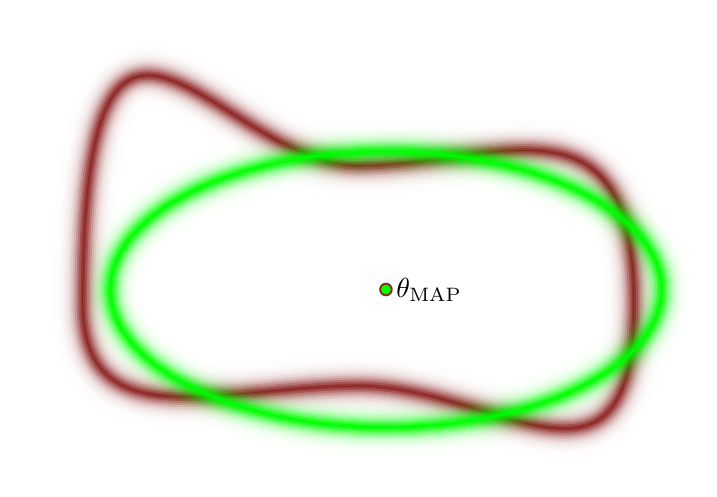
\begin{tikzpicture}[scale=0.35, thick]

  \begin{scope}
    \clip (-12, -6) rectangle (12, 10);
    \foreach \i in {0, 0.05,..., 1} {
      \draw[line width={30 * \i}, opacity={exp(-8 * \i)}, dark] 
        (-10, 0) .. controls (-10, 15) and (-5, 5) .. (0, 5)
        .. controls (5, 5) and (10, 8) .. (10, 0)
        .. controls (10, -8) and (5, -3) .. (0, -3)
        .. controls (-5, -3) and (-10, -5) .. (-10, 0);
    }  
    
    \foreach \i in {0, 0.05,..., 1} {
      \draw[line width={30 * \i}, opacity={exp(-8 * \i)}, green] 
        (1, 0.5) ellipse (10 and 5);
    }
  \end{scope}
 
  \fill[color=dark] (1, 0.5) circle (7pt);
  \fill[color=green] (1, 0.5) circle (5pt)
  node[right, color=black]  { $\theta_{\mathrm{MAP}}$ };
  
\end{tikzpicture}
\caption{For simple probability distributions with well-chosen
samples spaces, the local geometry around the mode of a 
probability density function can quantify the geometry of the 
entire typical set, yielding accurate Laplace estimators. For
more complex probability distributions, however, this local
information poorly quantifies the global geometry of the 
typical set and Laplace estimators suffer from large biases.
}
\label{fig:laplace}
\end{figure*}

As with the simpler MAP estimators, the dependence on the particular
sample space manifests as fragility of the corresponding estimators
and we have no generic means of quantifying the error in practice.  
If we want robust estimation of probabilities and expectations then we 
need strategies that do not depend on these irrelevant properties.

\subsection{Variational Estimators}

In order to construct a approximation that is not sensitive to the choice 
of a particular sample space we need to frame the problem as an 
optimization over a space of approximating distributions directly.
Optimizations over spaces of probability distributions fall into a class 
of algorithms known as \emph{variational methods}.

Variational methods are characterized by two choices: the variational
family and a divergence function. The \emph{variational family}, 
$\mathcal{Q}$, is a set of probability distributions over the target sample 
space, $\Theta$, such that at least some expectations can be computed
analytically.  In order to identify the best approximation to the target 
distribution we then define a \emph{divergence function},
%
\begin{align*}
D &: 
\mathcal{Q} \times \mathcal{Q}
\rightarrow \mathbb{R}^{+}
\\
& \quad \PP_{1}, \PP_{2} 
\mapsto D \! \left( \PP_{1} \mid\mid \PP_{2} \right),
\end{align*}
%
which is zero if the two arguments are the same and increases as they 
deviate from each other more strongly.

The best approximating distribution is then defined by the variational 
objective (Figure \ref{fig:variational_cartoon}).
%
\begin{equation*}
\mathbb{Q}^{*}
= 
\underset{\mathbb{Q} \in \mathcal{Q}}{\mathrm{argmin}} \,
D \! \left( \PP \mid\mid \mathbb{Q} \right).
\end{equation*}
%
Although straightforward to define, this variational optimization can
quite challenging in practice.  Depending on how the target distribution
interacts with the choice of variational distribution and divergence
function, the variational objective might feature multiple critical points
and we may not be able to find the global optimum in practice
(Figure \ref{fig:variational_challenges}).

\begin{figure*}
\centering
%
\subfigure[]{
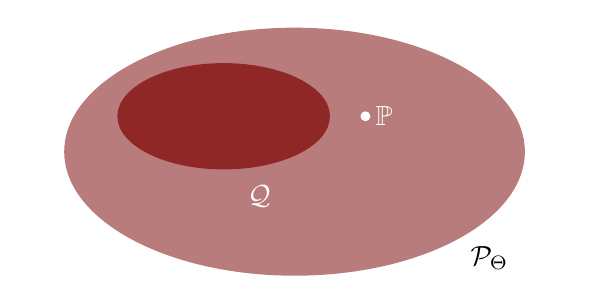
\begin{tikzpicture}[scale=0.225, thick]
  
  \draw[color=white] (-15, 0) -- (15, 0);
  
  \fill[mid] (0, 0) ellipse (13 and 7);
  \node at (11, -6) {$\mathcal{P}_{\Theta}$};
  
  \fill[dark] (-4, 2) ellipse (6 and 3);
  \node[color=white] at (-2, -2.5) {$\mathcal{Q}$};
  
  \fill[color=white] (4, 2) circle (8pt)
  node[right, color=white] {$\PP$};
  
\end{tikzpicture}
}
\subfigure[]{
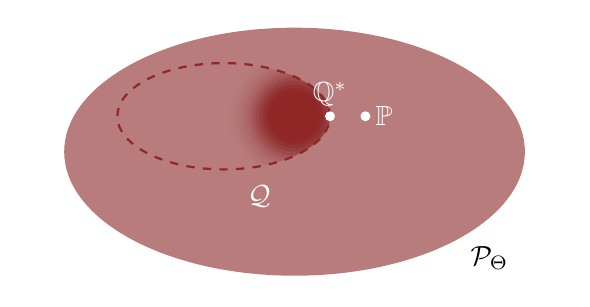
\begin{tikzpicture}[scale=0.225, thick]

  \draw[color=white] (-15, 0) -- (15, 0);
  
  \fill[mid] (0, 0) ellipse (13 and 7);
  \node at (11, -6) {$\mathcal{P}_{\Theta}$};
  
  \draw[color=dark, dashed] (-4, 2) ellipse (6 and 3);
  \node[color=white] at (-2, -2.5) {$\mathcal{Q}$};
  
  \begin{scope}
    \clip (-4, 2) ellipse (6 and 3);
    \foreach \i in {0, 0.05,..., 1} {
      \fill[opacity={exp(-5 * \i*\i)}, dark] (0, 2) circle ({4 * \i});      
    }
  \end{scope}
  
  \fill[color=white] (2, 2) circle (8pt)
  node[above, color=white] {$\mathbb{Q}^{*}$};
  
  \fill[color=white] (4, 2) circle (8pt)
  node[right, color=white] {$\PP$};
  
\end{tikzpicture}
}
\caption{(a) A variational family, $\mathcal{Q}$, is a set of probability distributions
over the same sample space, $\Theta$, as the target distribution,
$\PP$, taken from the set of all probability distributions over $\Theta$,
$\mathcal{P}_{\Theta}$.  (b) Adding a divergence function distinguishes which
elements of $\mathcal{Q}$ are good approximations to the target
distribution, allowing us to identify the best approximation, $\mathbb{Q}^{*}$.
}
\label{fig:variational_cartoon}
\end{figure*}

\begin{figure*}
\centering
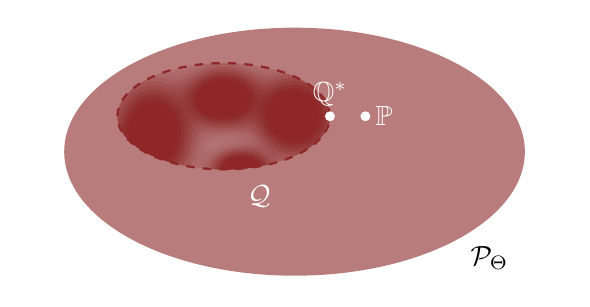
\begin{tikzpicture}[scale=0.225, thick]

  \draw[color=white] (-15, 0) -- (15, 0);
  
  \fill[mid] (0, 0) ellipse (13 and 7);
  \node at (11, -6) {$\mathcal{P}_{\Theta}$};
  
  \draw[color=dark, dashed] (-4, 2) ellipse (6 and 3);
  \node[color=white] at (-2, -2.5) {$\mathcal{Q}$};
  
  \begin{scope}
    \clip (-4, 2) ellipse (6 and 3);
    
    \foreach \i in {0, 0.05,..., 1} {
      \fill[opacity={exp(-5 * \i*\i)}, dark] (0, 2) circle ({4 * \i});      
    }
    
    \foreach \i in {0, 0.05,..., 1} {
      \fill[opacity={exp(-5 * \i*\i)}, dark] (-4, 3) ellipse ({4 * \i} and {3 * \i});      
    }
    
    \foreach \i in {0, 0.05,..., 1} {
      \fill[opacity={exp(-5 * \i*\i)}, dark] (-8, 1) ellipse ({4 * \i} and {5 * \i});      
    }
    
    \foreach \i in {0, 0.05,..., 1} {
      \fill[opacity={exp(-5 * \i*\i)}, dark] (-3, -1) ellipse ({3 * \i} and {2 * \i});      
    }
  \end{scope}
  
  \fill[color=white] (2, 2) circle (8pt)
  node[above, color=white] {$\mathbb{Q}^{*}$};
  
  \fill[color=white] (4, 2) circle (8pt)
  node[right, color=white] {$\PP$};
  
\end{tikzpicture}
\caption{In practice typically different elements of the variational family
are able to capture different characteristics of the target distribution and 
the variational objective manifests multiple optima.  Even if a global
optimum, $\mathbb{Q}^{*}$, exists it will be difficult to find and we may
be left with only a suboptimal local optimum.
}
\label{fig:variational_challenges}
\end{figure*}

Even if we could find the best approximating distribution, however,
there are no guarantees that it will yield accurate estimates for
all relevant expectations of our target distribution.  For example, 
some divergence functions are biased towards variational solutions
that underestimate the breadth of the typical set while others
tend to significantly overestimate it (Figure \ref{fig:variational_approximations}).

Variational methods are relatively new to statistics and at the moment
there are no generic methods for quantifying the error in variational
estimators.

\begin{figure*}
\centering
\subfigure[]{
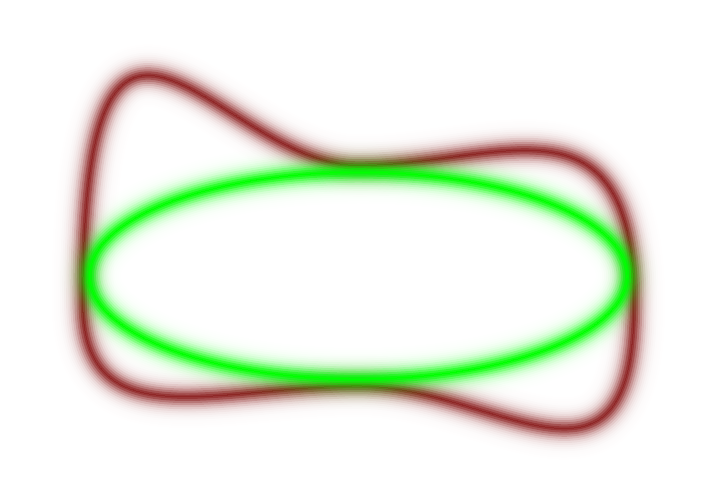
\begin{tikzpicture}[scale=0.35, thick]
  \begin{scope}
    \clip (-12, -6) rectangle (12, 10);
    \foreach \i in {0, 0.05,..., 1} {
      \draw[line width={30 * \i}, opacity={exp(-8 * \i)}, dark] 
        (-10, 0) .. controls (-10, 15) and (-5, 5) .. (0, 5)
        .. controls (5, 5) and (10, 8) .. (10, 0)
        .. controls (10, -8) and (5, -3) .. (0, -3)
        .. controls (-5, -3) and (-10, -5) .. (-10, 0);
    }  
    
    \foreach \i in {0, 0.05,..., 1} {
      \draw[line width={30 * \i}, opacity={exp(-8 * \i)}, green] 
        (0, 1) ellipse (9.75 and 3.75);
    }
  \end{scope}
\end{tikzpicture}
}
\subfigure[]{
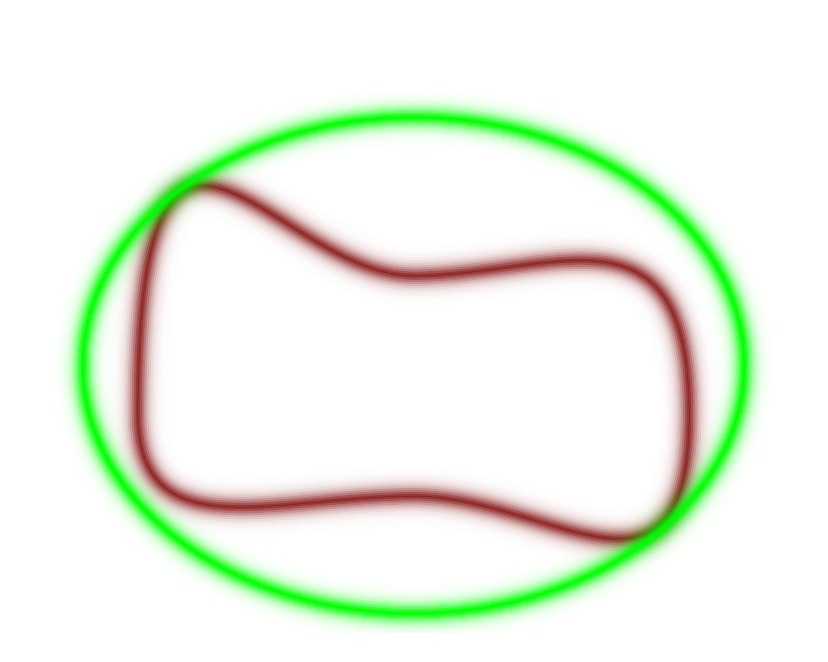
\begin{tikzpicture}[scale=0.35, thick]
  \begin{scope}
    \clip (-14, -8) rectangle (14, 14);
    \foreach \i in {0, 0.05,..., 1} {
      \draw[line width={30 * \i}, opacity={exp(-8 * \i)}, dark] 
        (-10, 0) .. controls (-10, 15) and (-5, 5) .. (0, 5)
        .. controls (5, 5) and (10, 8) .. (10, 0)
        .. controls (10, -8) and (5, -3) .. (0, -3)
        .. controls (-5, -3) and (-10, -5) .. (-10, 0);
    }  
    
    \foreach \i in {0, 0.05,..., 1} {
      \draw[line width={30 * \i}, opacity={exp(-8 * \i)}, green] 
        (0, 1.75) ellipse (12 and 9);
    }
  \end{scope}
\end{tikzpicture}
}
\caption{Intuition about the effects of a particular variational divergence 
function can be developed by considering how the typical set of an
approximating distribution (green) interacts with the typical of the target 
distribution (red).  (a) Some divergence functions favor approximating
distributions that expand into the interior of the target typical set,
resulting in an underestimate of the breadth of the typical set.  (b)
Others, however, favor approximating distractions that collapse around
the exterior of the target typical set, resulting in overestimated expectations.
}
\label{fig:variational_approximations}
\end{figure*}

\section{Probability in Practice: Stochastic Estimators}

The accuracy of deterministic estimators will always be limited by
the flexibility of the approximating distribution to match the geometry 
of the typical set of the target distribution.  The only way to overcome
this restriction is to quantify the typical set of the target distribution
directly.  Unfortunately, this presents problems of its own as in practice 
we don't know where to find the typical set in the expansive sample space.  Because exhaustive search of the sample space is far too expensive
we need a more targeted procedure for finding and then exploring 
the typical set.

By construction an infinite number of samples from the target distribution 
quantifies the typical set, and hence the samples themselves provide
a naturally way to identify the typical set (Figure \ref{fig:samples}).  The
utility of samples, however, depends both on how precisely we can 
quantify the typical set using only a finite number of samples and how
well we can generate samples in the first place.

\emph{Stochastic estimators} use samples, either from the target probability
distribution or auxiliary probability distributions, to construct estimators 
of the expectation with respect to the target distribution.  Exactly how these
samples are generated leads to estimators with substantially different 
behaviors.

\subsection{Monte Carlo Estimators}

Monte Carlo estimators use a finite sequence of exact samples from
the target distribution to estimate expectations.  Given a sequence
of exact samples $\left\{ \theta_{1}, \ldots, \theta_{N} \right\}$ we can
construct a  \emph{Monte Carlo estimator} of the expectation of 
\emph{any} function $f : \Theta \rightarrow \RR$ as
%
\begin{equation*}
\hat{f}^{\mathrm{MC}}_{N} \equiv
\frac{1}{N} \sum_{n = 1}^{N} f \! \left( \theta_{n} \right).
\end{equation*}

By construction these Monte Carlo estimators recover the exact
expectation asymptotically,
%
\begin{equation*}
\lim_{N \rightarrow \infty} \hat{f}^{\mathrm{MC}}_{N}
=
\EE_{\PP} [ f ],
\end{equation*}
%
but they are also accurate even when the sequence is finite.
Provided that the samples are exact, Monte Carlo estimators 
follow a Central Limit Theorem -- for sufficiently large $N$ the 
estimators themselves follow a distribution given by a Gaussian 
density,
%
\begin{equation*}
\hat{f}_{N} \sim 
\mathcal{N} \! \left( \EE_{\PP} [ f ],
\mathrm{MCSE} \right),
\end{equation*}
%
where the \emph{Monte Carlo Standard Error} is defined as
%
\begin{equation*}
\mathrm{MCSE } \equiv \sqrt{ \frac{ \mathrm{Var} [ f ] }{N} }.
\end{equation*}
%
Consequently Monte Carlo estimators are unbiased with respect
to all of the possible sequences we could have generated, and 
their precision improves as we generate more and more samples.
Moreover, functions with high variance are more challenging to
estimate than those with low variance.

In practice we use another Monte Carlo estimator to approximate the
variance $\mathrm{Var} [ f ] $, and hence the Monte Carlo Standard
Error itself.  The error of this approximation is $\mathrm{Var} [ \,
\mathrm{Var} [ f ]  \, ] / N$ which is typically negligible compared to
the Monte Carlo Standard Error of $f$.  Monte Carlo estimators, then,
are distinct from deterministic approximations in that they naturally
come equipped with a procedure for at least estimating their error.

Of course all of these benefits of Monte Carlo estimators are dependent 
on our ability to generate exact samples from the target probability 
distribution.  Unfortunately, generating exact samples is infeasible for all 
but the simplest probability distributions, and we are once again frustrated 
by our ignorance of the typical set.  In order to proceed we need to 
approximate exact samples themselves.

\subsection{Importance Sampling Estimators}

Although we typically can't generate exact samples from the target 
distribution, often we can generate exact samples from an 
\emph{auxiliary} probability distribution, $\mathbb{G}$,
%
\begin{equation*}
\left\{ \vartheta_{1}, \ldots, \vartheta_{N} \right\} \sim \mathbb{G}.
\end{equation*}
%
\emph{Importance sampling estimators} use these auxiliary samples 
corrected with \emph{importance weights}, $w \! \left( \vartheta \right)$,  
%
\begin{equation*}
\EE_{\PP} [ f ] \approx 
\hat{f}^{\mathrm{IS}}_{N} = 
\frac{1}{N} \sum_{n = 1}^{N} 
w \! \left( \vartheta_{n} \right) f \! \left( \vartheta_{n} \right)
\end{equation*}
%
If $p$ and $g$ are the probability density functions corresponding to
the target distribution and auxiliary distribution, respectively, then the 
importance weights are given by
%
\begin{equation*}
w \! \left( \vartheta_{n} \right) =
\frac{ p \! \left( \vartheta_{n} \right) }
{ g \! \left( \theta_{n} \right) }.
\end{equation*}
%
Although they are constructed from probability density functions, 
impotence weights, and hence importance sampling estimators,
are invariant to the choice of sample space.  When we map to
an equivalent sample space, the resulting Jacobian is the same
in both the numerator and denominator and hence cancels when
evaluating the weights themselves.

Given certain regularity conditions, importance sampling estimators 
also satisfy a Central Limit Theorem
%
\begin{equation*}
\hat{f}_{N}^{\mathrm{IS}} \sim 
\mathcal{N} \! \left( \EE_{\PP} [ f ],
\mathrm{ISSE} \right),
\end{equation*}
%
The \emph{Importance Sampling Standard Error} is given by
%
\begin{equation*}
\mathrm{ISSE} \equiv \sqrt{ \frac{ \mathrm{Var} [ f ] }{\mathrm{ESS} } },
\end{equation*}
%
with the \emph{effective sample size} defined as
%
\begin{equation*}
\mathrm{ESS} = 
N 
\frac{ \left( \sum_{n = 1}^{N} w \! \left( \vartheta_{n} \right) \right)^{2} }
{ \sum_{n = 1}^{N} w \! \left( \vartheta_{n} \right)^{2} }.
\end{equation*}
%
Comparing this to the Monte Carlo Central Limit Theorem we can
see that the effective sample size quantifies how many exact
samples would have yielded the same estimator precision,
hence the effective sample size can be interpreted as the
effective number of exact samples ``contained'' in the auxiliary
samples.

The challenge with constructing a useful importance sampler is
finding an auxiliary distribution that is not too different from the
target distribution.  Although importance sampling estimators are 
unbiased, their variance can be so large as to be impractical when 
the auxiliary distribution deviates too strongly from the target distribution 
and the weights are large.  In fact, when the auxiliary distribution has 
lighter tails than the target distribution these estimators can 
easily have infinitely large variance: not only does this make 
the estimators themselves useless, it also makes estimates of 
the variance and hence any quantification of the estimator error 
useless.

Selecting an auxiliary distribution that yields accurate importance
sampler estimators, however, is challenging without knowing
the structure of the typical set a priori.  Ultimately, importance
sampling is most useful as a means to correct a distribution that 
is already known to be a good approximation to the target
distribution.

\subsection{Markov Chain Monte Carlo Estimators}

Another strategy for approximating the Monte Carlo procedure
is to generate samples from the target distribution but relax
the requirement that they be exact.  Fortunately, correlated 
samples are readily given by \emph{Markov chains}.

A Markov chain is a stochastic processes generated not by 
static probability distribution but by a probability distribution 
that depends on the last state in the sequence.  In other words, 
each state in the sequence is sampled from a conditional 
probability distribution known as a \emph{Markov transition 
kernel}, $\mathbb{T}$, 
%
\begin{align*}
\mathbb{T}
&: \EV{\Theta} \times \Theta \rightarrow \left[0, 1 \right] \\
&\quad \left( E, \theta \right) \;\; \mapsto 
\mathbb{T} \! \left[ E \mid \theta \right].
\end{align*}
%
When the Markov transition operator preserves the target
distribution,
%
\begin{equation*}
\PP \! \left[ E \right]
=
\mathbb{E}_{\PP} \! 
\left[  \mathbb{T} \! \left[ E \mid \theta \right] \right]
\end{equation*}
%
or, with respect to probability density functions,
%
\begin{equation*}
p \! \left( \theta \right)
=
\int_{\Theta} t \! \left( \theta' \mid \theta \right) 
\pi \! \left( \theta' \right) \dd \theta',
\end{equation*}
%
then the Markov chain asymptotically recovers expectations
with \emph{Markov chain Monte Carlo estimators},
%
\begin{equation*}
\lim_{N \rightarrow \infty} 
\hat{f}^{\mathrm{MCMC}}_{N}
\equiv
\lim_{N \rightarrow \infty} 
\frac{1}{N} \sum_{n = 1}^{N} f \! \left( \theta_{n} \right)
=
\mathbb{E}_{\PP} \! \left[ f \right],
\end{equation*}
%
and we can interpret the Markov chain itself as a sequence
of correlated samples from the target distribution.

More intuitively, the Markov transition kernel quantifies
the variability in each step of the Markov chain.  When the
transition preserves the target distribution, then it 
concentrates closer to the typical set than away from it --
it is literally attracted to the typical set.  Consequently, the
Markov chain will eventually find and then explore the
typical set no matter where we start in the sample space,
and the Markov chain Monte Carlo estimators will converge
to the true expectations.
 
The important caveat here is that the Markov chain is 
guaranteed to find and full explore the typical set only 
asymptotically.  In practice, however, it is the only the finite time 
performance of Markov chains that matters.  Unfortunately, the 
finite time behavior of Markov chain Monte Carlo is much more
subtle than its exact predecessor.

In this section we discuss how Markov chain Monte Carlo
behaves under ideal conditions, how it behaves under
less-than-ideal conditions, and how to effectively run
the algorithm in practice to be robust to the latter.

\subsubsection{Markov Chain Monte Carlo Under Ideal Conditions}

Under ideal conditions, Markov chains explore the target
distribution in three distinct phases.  In the first phase the
Markov chain converges towards the typical set from its
initial position and Markov chain Monte Carlo estimators
are highly biased (Figure \ref{fig:ideal_mcmc}a).  The
second phase begins once the Markov chain finds the
typical set and persists through the first sojourn across
the typical set.  This initial exploration is extremely effective
and the accuracy of Markov chain Monte Carlo estimators
rapidly improves (Figure \ref{fig:ideal_mcmc}b).  The
third phase consists of all subsequent exploration where
the the Markov chain refines its exploration of the typical
set and the precision of the Markov chain Monte Carlo 
estimators improves, albeit at a slower rate (Figure 
\ref{fig:ideal_mcmc}c).

\begin{figure*}
\centering
\subfigure[]{
\begin{tikzpicture}[scale=0.25, thick]
  \draw[-,color=white] (-12, 0) to (12, 0);
  
  \begin{scope}
  \clip (-12, -10) rectangle (12, 10);
  
  \foreach \i in {0, 0.05,..., 1} {
    \draw[line width={30 * \i}, opacity={exp(-8 * \i)}, dark] 
      (-10, 0) .. controls (-10, 15) and (-5, 5) .. (0, 5)
      .. controls (5, 5) and (10, 8) .. (10, 0)
      .. controls (10, -8) and (5, -3) .. (0, -3)
      .. controls (-5, -3) and (-10, -5) .. (-10, 0);
  }

  %\fill[color=dark] (-11, -8) circle (7pt);  
  %\fill[color=light] (-11, -8) circle (5pt);
  
  \fill[color=dark] (-10, -6.5) circle (7pt);  
  \fill[color=light] (-10, -6.5) circle (5pt);
  
  \fill[color=dark] (-9, -6.75) circle (7pt);  
  \fill[color=light] (-9, -6.75) circle (5pt);
  
  \fill[color=dark] (-8.25, -5) circle (7pt);  
  \fill[color=light] (-8.25, -5) circle (5pt);
  
  \fill[color=dark] (-7.5, -4) circle (7pt);  
  \fill[color=light] (-7.5, -4) circle (5pt);
  
  \fill[color=dark] (-7, -3.5) circle (7pt);  
  \fill[color=light] (-7, -3.5) circle (5pt);
  
  \fill[color=dark] (-6.5, -3.6) circle (7pt);  
  \fill[color=light] (-6.5, -3.6) circle (5pt);  
  
  \end{scope}
  
  \draw[-,color=white] (14, 0) to (38, 0);  
  \node[] at (28,3) {\includegraphics[width=5cm]{convergence1.eps}};
  \node[rotate=90] at (15.5,3) { $\left| \mathbb{E} \! \left[ f \right] - \hat{f} \right|$ };
\end{tikzpicture}
}
\subfigure[]{
\begin{tikzpicture}[scale=0.25, thick]
  \draw[-,color=white] (-12, 0) to (12, 0);
  
  \begin{scope}
  \clip (-12, -10) rectangle (12, 10);
  \foreach \i in {0, 0.05,..., 1} {
    \draw[line width={30 * \i}, opacity={exp(-8 * \i)}, dark] 
      (-10, 0) .. controls (-10, 15) and (-5, 5) .. (0, 5)
      .. controls (5, 5) and (10, 8) .. (10, 0)
      .. controls (10, -8) and (5, -3) .. (0, -3)
      .. controls (-5, -3) and (-10, -5) .. (-10, 0);
  }
  
  % Convergence
  
  %\fill[color=dark] (-11, -8) circle (7pt);  
  %\fill[color=light] (-11, -8) circle (5pt);
  
  \fill[color=dark] (-10, -6.5) circle (7pt);  
  \fill[color=light] (-10, -6.5) circle (5pt);
  
  \fill[color=dark] (-9, -6.75) circle (7pt);  
  \fill[color=light] (-9, -6.75) circle (5pt);
  
  \fill[color=dark] (-8.25, -5) circle (7pt);  
  \fill[color=light] (-8.25, -5) circle (5pt);
  
  \fill[color=dark] (-7.5, -4) circle (7pt);  
  \fill[color=light] (-7.5, -4) circle (5pt);
  
  \fill[color=dark] (-7, -3.5) circle (7pt);  
  \fill[color=light] (-7, -3.5) circle (5pt);
  
  \fill[color=dark] (-6.5, -3.6) circle (7pt);  
  \fill[color=light] (-6.5, -3.6) circle (5pt);  
  
  % Mixing
  
  \fill[color=dark] (-6, -3) circle (7pt);  
  \fill[color=light] (-6, -3) circle (5pt);
  
  %\fill[color=dark] (-5.5, -3.5) circle (7pt);  
  %\fill[color=light] (-5.5, -3.5) circle (5pt);
  
  %\fill[color=dark] (-5, -3.75) circle (7pt);  
  %\fill[color=light] (-5, -3.75) circle (5pt);
  
  \fill[color=dark] (-4.75, -3.25) circle (7pt);  
  \fill[color=light] (-4.75, -3.25) circle (5pt);
  
  %\fill[color=dark] (-5, -3.5) circle (7pt);  
  %\fill[color=light] (-5, -3.5) circle (5pt);  
  
  %\fill[color=dark] (-4, -3.8) circle (7pt);  
  %\fill[color=light] (-4, -3.8) circle (5pt);
  
  \fill[color=dark] (-3, -3.5) circle (7pt);  
  \fill[color=light] (-3, -3.5) circle (5pt);
  
  %\fill[color=dark] (-2.8, -3) circle (7pt);  
  %\fill[color=light] (-2.8, -3) circle (5pt);
  
  %\fill[color=dark] (-2.9, -3.3) circle (7pt);  
  %\fill[color=light] (-2.9, -3.3) circle (5pt);  
  
  \fill[color=dark] (-2, -3.5) circle (7pt);  
  \fill[color=light] (-2, -3.5) circle (5pt);
  
  %\fill[color=dark] (-1.25, -3) circle (7pt);  
  %\fill[color=light] (-1.25, -3) circle (5pt);
  
  %\fill[color=dark] (-0.5, -2.75) circle (7pt);  
  %\fill[color=light] (-0.5, -2.75) circle (5pt);
  
  \fill[color=dark] (-0.3, -3) circle (7pt);  
  \fill[color=light] (-0.3, -3) circle (5pt);  
  
  %\fill[color=dark] (0.1, -2.75) circle (7pt);  
  %\fill[color=light] (0.1, -2.75) circle (5pt);
  
  %\fill[color=dark] (0.15, -3.1) circle (7pt);  
  %\fill[color=light] (0.15, -3.1) circle (5pt);  
  
  \fill[color=dark] (0.4, -3.4) circle (7pt);  
  \fill[color=light] (0.4, -3.4) circle (5pt);
  
  %\fill[color=dark] (1.1, -3.25) circle (7pt);  
  %\fill[color=light] (1.1, -3.25) circle (5pt);
  
  %\fill[color=dark] (2.7, -3.45) circle (7pt);  
  %\fill[color=light] (2.7, -3.45) circle (5pt);
  
  \fill[color=dark] (2.9, -3.2) circle (7pt);  
  \fill[color=light] (2.9, -3.2) circle (5pt);
  
  %\fill[color=dark] (3.1, -3.7) circle (7pt);  
  %\fill[color=light] (3.1, -3.7) circle (5pt);
  
  %\fill[color=dark] (4.2, -3.9) circle (7pt);  
  %\fill[color=light] (4.2, -3.9) circle (5pt);
  
  \fill[color=dark] (4, -4.1) circle (7pt);  
  \fill[color=light] (4, -4.1) circle (5pt);
  
  %\fill[color=dark] (5, -4) circle (7pt);  
  %\fill[color=light] (5, -4) circle (5pt);
  
  %\fill[color=dark] (5.8, -4.3) circle (7pt);  
  %\fill[color=light] (5.8, -4.3) circle (5pt);
  
  \fill[color=dark] (6.5, -4.8) circle (7pt);  
  \fill[color=light] (6.5, -4.8) circle (5pt);
  
  %\fill[color=dark] (6.8, -4.5) circle (7pt);  
  %\fill[color=light] (6.8, -4.5) circle (5pt);
  
  %\fill[color=dark] (7, -4.6) circle (7pt);  
  %\fill[color=light] (7, -4.6) circle (5pt);
  
  \fill[color=dark] (6.8, -4.7) circle (7pt);  
  \fill[color=light] (6.8, -4.7) circle (5pt);
  
  %\fill[color=dark] (7.75, -4.2) circle (7pt);  
  %\fill[color=light] (7.75, -4.2) circle (5pt);
  
  %\fill[color=dark] (8.5, -4.25) circle (7pt);  
  %\fill[color=light] (8.5, -4.25) circle (5pt);
  
  \fill[color=dark] (8.6, -4.75) circle (7pt);  
  \fill[color=light] (8.6, -4.75) circle (5pt);
  
  %\fill[color=dark] (8.8, -4.5) circle (7pt);  
  %\fill[color=light] (8.8, -4.5) circle (5pt);
  
  %\fill[color=dark] (9.25, -3.5) circle (7pt);  
  %\fill[color=light] (9.25, -3.5) circle (5pt);
  
  \fill[color=dark] (9.65, -2.75) circle (7pt);  
  \fill[color=light] (9.65, -2.75) circle (5pt);
  
  %\fill[color=dark] (9.5, -2) circle (7pt);  
  %\fill[color=light] (9.5, -2) circle (5pt);

  %\fill[color=dark] (9.8, -3) circle (7pt);  
  %\fill[color=light] (9.8, -3) circle (5pt);
  
  \fill[color=dark] (9.85, -0.8) circle (7pt);  
  \fill[color=light] (9.85, -0.8) circle (5pt);
  
  %\fill[color=dark] (10.1, -0.4) circle (7pt);  
  %\fill[color=light] (10.1, -0.4) circle (5pt);

  %\fill[color=dark] (10.25, 0.3) circle (7pt);  
  %\fill[color=light] (10.25, 0.3) circle (5pt);
  
  \fill[color=dark] (10, 0.7) circle (7pt);  
  \fill[color=light] (10, 0.7) circle (5pt);
  
  %\fill[color=dark] (9.7, 0.9) circle (7pt);  
  %\fill[color=light] (9.7, 0.9) circle (5pt);
  
  %\fill[color=dark] (10.3, 1.4) circle (7pt);  
  %\fill[color=light] (10.3, 1.4) circle (5pt);
  
  \fill[color=dark] (9.8, 2.25) circle (7pt);  
  \fill[color=light] (9.8, 2.25) circle (5pt);
  
  %\fill[color=dark] (10, 2.5) circle (7pt);  
  %\fill[color=light] (10, 2.5) circle (5pt);
  
  %\fill[color=dark] (10, 3) circle (7pt);  
  %\fill[color=light] (10, 3) circle (5pt);
  
  \fill[color=dark] (9.6, 3.75) circle (7pt);  
  \fill[color=light] (9.6, 3.75) circle (5pt);
  
  %\fill[color=dark] (9.1, 4.4) circle (7pt);  
  %\fill[color=light] (9.1, 4.4) circle (5pt);
  
  %\fill[color=dark] (9.1, 4.1) circle (7pt);  
  %\fill[color=light] (9.1, 4.1) circle (5pt);
  
  \fill[color=dark] (8.5, 4.75) circle (7pt);  
  \fill[color=light] (8.5, 4.75) circle (5pt);
  
  %\fill[color=dark] (8.1, 5.75) circle (7pt);  
  %\fill[color=light] (8.1, 5.75) circle (5pt);
  
  %\fill[color=dark] (7.7, 5.2) circle (7pt);  
  %\fill[color=light] (7.7, 5.2) circle (5pt);
  
  \fill[color=dark] (7.3, 5.3) circle (7pt);  
  \fill[color=light] (7.3, 5.3) circle (5pt);
  
  %\fill[color=dark] (6.6, 5.8) circle (7pt);  
  %\fill[color=light] (6.6, 5.8) circle (5pt);
  
  %\fill[color=dark] (6, 6) circle (7pt);  
  %\fill[color=light] (6, 6) circle (5pt);
  
  \fill[color=dark] (5.25, 5.45) circle (7pt);  
  \fill[color=light] (5.25, 5.45) circle (5pt);
  
  %\fill[color=dark] (4.75, 5.75) circle (7pt);  
  %\fill[color=light] (4.75, 5.75) circle (5pt);
  
  %\fill[color=dark] (3.5, 5.28) circle (7pt);  
  %\fill[color=light] (3.5, 5.28) circle (5pt);
  
  \fill[color=dark] (5, 5.65) circle (7pt);  
  \fill[color=light] (5, 5.65) circle (5pt);
  
  %\fill[color=dark] (3, 5.5) circle (7pt);  
  %\fill[color=light] (3, 5.5) circle (5pt);
  
  %\fill[color=dark] (2.75, 5.3) circle (7pt);  
  %\fill[color=light] (2.75, 5.3) circle (5pt);
  
  \fill[color=dark] (2.25, 4.8) circle (7pt);  
  \fill[color=light] (2.25, 4.8) circle (5pt);
  
  %\fill[color=dark] (2, 5.2) circle (7pt);  
  %\fill[color=light] (2, 5.2) circle (5pt);
  
  %\fill[color=dark] (1.75, 4.9) circle (7pt);  
  %\fill[color=light] (1.75, 4.9) circle (5pt);
  
  \fill[color=dark] (1.5, 5.1) circle (7pt);  
  \fill[color=light] (1.5, 5.1) circle (5pt);
  
  %\fill[color=dark] (0.8, 5.2) circle (7pt);  
  %\fill[color=light] (0.8, 5.2) circle (5pt);
 
  %\fill[color=dark] (0, 4.7) circle (7pt);  
  %\fill[color=light] (0, 4.7) circle (5pt);
  
  \fill[color=dark] (-0.6, 5) circle (7pt);  
  \fill[color=light] (-0.6, 5) circle (5pt);
  
  %\fill[color=dark] (-1.25, 5.2) circle (7pt);  
  %\fill[color=light] (-1.25, 5.2) circle (5pt);
  
  %\fill[color=dark] (-1.55, 5.4) circle (7pt);  
  %\fill[color=light] (-1.55, 5.4) circle (5pt);
  
  \fill[color=dark] (-1.85, 5) circle (7pt);  
  \fill[color=light] (-1.85, 5) circle (5pt);
  
  %\fill[color=dark] (-2.75, 5.5) circle (7pt);  
  %\fill[color=light] (-2.75, 5.5) circle (5pt);
  
  %\fill[color=dark] (-3.5, 6.6) circle (7pt);  
  %\fill[color=light] (-3.5, 6.6) circle (5pt);
  
  \fill[color=dark] (-4.25, 6.5) circle (7pt);  
  \fill[color=light] (-4.25, 6.5) circle (5pt);
  
  %\fill[color=dark] (-4.9, 7.2) circle (7pt);  
  %\fill[color=light] (-4.9, 7.2) circle (5pt);
  
  %\fill[color=dark] (-5.2, 7) circle (7pt);  
  %\fill[color=light] (-5.2, 7) circle (5pt);
  
  \fill[color=dark] (-5.75, 7.4) circle (7pt);  
  \fill[color=light] (-5.75, 7.4) circle (5pt);
  
  %\fill[color=dark] (-6, 7.9) circle (7pt);  
  %\fill[color=light] (-6, 7.9) circle (5pt);
  
  %\fill[color=dark] (-6.25, 7.8) circle (7pt);  
  %\fill[color=light] (-6.25, 7.8) circle (5pt);
  
  \fill[color=dark] (-6.5, 7.5) circle (7pt);  
  \fill[color=light] (-6.5, 7.5) circle (5pt);
  
  %\fill[color=dark] (-6.75, 8) circle (7pt);  
  %\fill[color=light] (-6.75, 8) circle (5pt);
  
  %\fill[color=dark] (-7.5, 8.5) circle (7pt);  
  %\fill[color=light] (-7.5, 8.5) circle (5pt);
  
  \fill[color=dark] (-8.25, 8) circle (7pt);  
  \fill[color=light] (-8.25, 8) circle (5pt);
  
  %\fill[color=dark] (-8.65, 7.8) circle (7pt);  
  %\fill[color=light] (-8.65, 7.8) circle (5pt);
  
  %\fill[color=dark] (-8.4, 7.7) circle (7pt);  
  %\fill[color=light] (-8.4, 7.7) circle (5pt);
  
  \fill[color=dark] (-9.2, 7) circle (7pt);  
  \fill[color=light] (-9.2, 7) circle (5pt);
  
  %\fill[color=dark] (-9.5, 6.75) circle (7pt);  
  %\fill[color=light] (-9.5, 6.75) circle (5pt);
  
  %\fill[color=dark] (-10, 6) circle (7pt);  
  %\fill[color=light] (-10, 6) circle (5pt);
  
  \fill[color=dark] (-9.7, 5.3) circle (7pt);  
  \fill[color=light] (-9.7, 5.3) circle (5pt);
  
  %\fill[color=dark] (-9.6, 5) circle (7pt);  
  %\fill[color=light] (-9.6, 5) circle (5pt);
  
  %\fill[color=dark] (-9.9, 4.75) circle (7pt);  
  %\fill[color=light] (-9.9, 4.75) circle (5pt);
  
  \fill[color=dark] (-10.1, 4) circle (7pt);  
  \fill[color=light] (-10.1, 4) circle (5pt);
  
  %\fill[color=dark] (-9.7, 3.5) circle (7pt);  
  %\fill[color=light] (-9.7, 3.5) circle (5pt);
  
  %\fill[color=dark] (-9.8, 3) circle (7pt);  
  %\fill[color=light] (-9.8, 3) circle (5pt);
  
  \fill[color=dark] (-10, 2.2) circle (7pt);  
  \fill[color=light] (-10, 2.2) circle (5pt);  
  
  %\fill[color=dark] (-10.25, 1.9) circle (7pt);  
  %\fill[color=light] (-10.25, 1.9) circle (5pt);  
  
  %\fill[color=dark] (-9.7, 1.8) circle (7pt);  
  %\fill[color=light] (-9.7, 1.8) circle (5pt);  
  
  \fill[color=dark] (-10.2, 1.4) circle (7pt);  
  \fill[color=light] (-10.2, 1.4) circle (5pt);  
  
  %\fill[color=dark] (-9.8, 0.7) circle (7pt);  
  %\fill[color=light] (-9.8, 0.7) circle (5pt);  
  
  %\fill[color=dark] (-10.2, 0.1) circle (7pt);  
  %\fill[color=light] (-10.2, 0.1) circle (5pt);  
  
  \fill[color=dark] (-9.9, -0.1) circle (7pt);  
  \fill[color=light] (-9.9, -0.1) circle (5pt);  
  
  %\fill[color=dark] (-10, -0.9) circle (7pt);  
  %\fill[color=light] (-10, -0.9) circle (5pt);  
  
  %\fill[color=dark] (-9.6, -1.5) circle (7pt);  
  %\fill[color=light] (-9.6, -1.5) circle (5pt);  
  
  \fill[color=dark] (-9.5, -1.8) circle (7pt);  
  \fill[color=light] (-9.5, -1.8) circle (5pt);  
  
  %\fill[color=dark] (-9.7, -2.1) circle (7pt);  
  %\fill[color=light] (-9.7, -2.1) circle (5pt);  
  
  %\fill[color=dark] (-9.3, -2.8) circle (7pt);  
  %\fill[color=light] (-9.3, -2.8) circle (5pt);  
  
  \fill[color=dark] (-8.3, -3) circle (7pt);  
  \fill[color=light] (-8.3, -3) circle (5pt);  
  
  %\fill[color=dark] (-7.8, -3.4) circle (7pt);  
  %\fill[color=light] (-7.8, -3.4) circle (5pt);  
  
  %\fill[color=dark] (-7.6, -3) circle (7pt);  
  %\fill[color=light] (-7.6, -3) circle (5pt);   
  
  \end{scope}
  
  \draw[-,color=white] (14, 0) to (38, 0);  
  \node[] at (28,3) {\includegraphics[width=5cm]{convergence2.eps}};
  \node[rotate=90] at (15.5,3) { $\left| \mathbb{E} \! \left[ f \right] - \hat{f} \right|$ };
\end{tikzpicture}
}
\subfigure[]{
\begin{tikzpicture}[scale=0.25, thick]
  \draw[-,color=white] (-12, 0) to (12, 0);
  
  \begin{scope}
  \clip (-12, -10) rectangle (12, 10);
  \foreach \i in {0, 0.05,..., 1} {
    \draw[line width={30 * \i}, opacity={exp(-8 * \i)}, dark] 
      (-10, 0) .. controls (-10, 15) and (-5, 5) .. (0, 5)
      .. controls (5, 5) and (10, 8) .. (10, 0)
      .. controls (10, -8) and (5, -3) .. (0, -3)
      .. controls (-5, -3) and (-10, -5) .. (-10, 0);
  }
  
  %\fill[color=dark] (-11, -8) circle (7pt);  
  %\fill[color=light] (-11, -8) circle (5pt);
  
  \fill[color=dark] (-10, -6.5) circle (7pt);  
  \fill[color=light] (-10, -6.5) circle (5pt);
  
  \fill[color=dark] (-9, -6.75) circle (7pt);  
  \fill[color=light] (-9, -6.75) circle (5pt);
  
  \fill[color=dark] (-8.25, -5) circle (7pt);  
  \fill[color=light] (-8.25, -5) circle (5pt);
  
  \fill[color=dark] (-7.5, -4) circle (7pt);  
  \fill[color=light] (-7.5, -4) circle (5pt);
  
  \fill[color=dark] (-7, -3.5) circle (7pt);  
  \fill[color=light] (-7, -3.5) circle (5pt);
  
  \fill[color=dark] (-6.5, -3.6) circle (7pt);  
  \fill[color=light] (-6.5, -3.6) circle (5pt);  
  
  \fill[color=dark] (-6, -3) circle (7pt);  
  \fill[color=light] (-6, -3) circle (5pt);
  
  \fill[color=dark] (-5.5, -3.5) circle (7pt);  
  \fill[color=light] (-5.5, -3.5) circle (5pt);
  
  \fill[color=dark] (-5, -3.75) circle (7pt);  
  \fill[color=light] (-5, -3.75) circle (5pt);
  
  \fill[color=dark] (-4.75, -3.25) circle (7pt);  
  \fill[color=light] (-4.75, -3.25) circle (5pt);
  
  \fill[color=dark] (-5, -3.5) circle (7pt);  
  \fill[color=light] (-5, -3.5) circle (5pt);  
  
  \fill[color=dark] (-4, -3.8) circle (7pt);  
  \fill[color=light] (-4, -3.8) circle (5pt);
  
  \fill[color=dark] (-3, -3.5) circle (7pt);  
  \fill[color=light] (-3, -3.5) circle (5pt);
  
  \fill[color=dark] (-2.8, -3) circle (7pt);  
  \fill[color=light] (-2.8, -3) circle (5pt);
  
  \fill[color=dark] (-2.9, -3.3) circle (7pt);  
  \fill[color=light] (-2.9, -3.3) circle (5pt);  
  
  \fill[color=dark] (-2, -3.5) circle (7pt);  
  \fill[color=light] (-2, -3.5) circle (5pt);
  
  \fill[color=dark] (-1.25, -3) circle (7pt);  
  \fill[color=light] (-1.25, -3) circle (5pt);
  
  \fill[color=dark] (-0.5, -2.75) circle (7pt);  
  \fill[color=light] (-0.5, -2.75) circle (5pt);
  
  \fill[color=dark] (-0.3, -3) circle (7pt);  
  \fill[color=light] (-0.3, -3) circle (5pt);  
  
  \fill[color=dark] (0.1, -2.75) circle (7pt);  
  \fill[color=light] (0.1, -2.75) circle (5pt);
  
  \fill[color=dark] (0.15, -3.1) circle (7pt);  
  \fill[color=light] (0.15, -3.1) circle (5pt);  
  
  \fill[color=dark] (0.4, -3.4) circle (7pt);  
  \fill[color=light] (0.4, -3.4) circle (5pt);
  
  \fill[color=dark] (1.1, -3.25) circle (7pt);  
  \fill[color=light] (1.1, -3.25) circle (5pt);
  
  \fill[color=dark] (2.7, -3.45) circle (7pt);  
  \fill[color=light] (2.7, -3.45) circle (5pt);
  
  \fill[color=dark] (2.9, -3.2) circle (7pt);  
  \fill[color=light] (2.9, -3.2) circle (5pt);
  
  \fill[color=dark] (3.1, -3.7) circle (7pt);  
  \fill[color=light] (3.1, -3.7) circle (5pt);
  
  \fill[color=dark] (4.2, -3.9) circle (7pt);  
  \fill[color=light] (4.2, -3.9) circle (5pt);
  
  \fill[color=dark] (4, -4.1) circle (7pt);  
  \fill[color=light] (4, -4.1) circle (5pt);
  
  \fill[color=dark] (5, -4) circle (7pt);  
  \fill[color=light] (5, -4) circle (5pt);
  
  \fill[color=dark] (5.8, -4.3) circle (7pt);  
  \fill[color=light] (5.8, -4.3) circle (5pt);
  
  \fill[color=dark] (6.5, -4.8) circle (7pt);  
  \fill[color=light] (6.5, -4.8) circle (5pt);
  
  \fill[color=dark] (6.8, -4.5) circle (7pt);  
  \fill[color=light] (6.8, -4.5) circle (5pt);
  
  \fill[color=dark] (7, -4.6) circle (7pt);  
  \fill[color=light] (7, -4.6) circle (5pt);
  
  \fill[color=dark] (6.8, -4.7) circle (7pt);  
  \fill[color=light] (6.8, -4.7) circle (5pt);
  
  \fill[color=dark] (7.75, -4.2) circle (7pt);  
  \fill[color=light] (7.75, -4.2) circle (5pt);
  
  \fill[color=dark] (8.5, -4.25) circle (7pt);  
  \fill[color=light] (8.5, -4.25) circle (5pt);
  
  \fill[color=dark] (8.6, -4.75) circle (7pt);  
  \fill[color=light] (8.6, -4.75) circle (5pt);
  
  \fill[color=dark] (8.8, -4.5) circle (7pt);  
  \fill[color=light] (8.8, -4.5) circle (5pt);
  
  \fill[color=dark] (9.25, -3.5) circle (7pt);  
  \fill[color=light] (9.25, -3.5) circle (5pt);
  
  \fill[color=dark] (9.65, -2.75) circle (7pt);  
  \fill[color=light] (9.65, -2.75) circle (5pt);
  
  \fill[color=dark] (9.5, -2) circle (7pt);  
  \fill[color=light] (9.5, -2) circle (5pt);

  \fill[color=dark] (9.8, -3) circle (7pt);  
  \fill[color=light] (9.8, -3) circle (5pt);
  
  \fill[color=dark] (9.85, -0.8) circle (7pt);  
  \fill[color=light] (9.85, -0.8) circle (5pt);
  
  \fill[color=dark] (10.1, -0.4) circle (7pt);  
  \fill[color=light] (10.1, -0.4) circle (5pt);

  \fill[color=dark] (10.25, 0.3) circle (7pt);  
  \fill[color=light] (10.25, 0.3) circle (5pt);
  
  \fill[color=dark] (10, 0.7) circle (7pt);  
  \fill[color=light] (10, 0.7) circle (5pt);
  
  \fill[color=dark] (9.7, 0.9) circle (7pt);  
  \fill[color=light] (9.7, 0.9) circle (5pt);
  
  \fill[color=dark] (10.3, 1.4) circle (7pt);  
  \fill[color=light] (10.3, 1.4) circle (5pt);
  
  \fill[color=dark] (9.8, 2.25) circle (7pt);  
  \fill[color=light] (9.8, 2.25) circle (5pt);
  
  \fill[color=dark] (10, 2.5) circle (7pt);  
  \fill[color=light] (10, 2.5) circle (5pt);
  
  \fill[color=dark] (10, 3) circle (7pt);  
  \fill[color=light] (10, 3) circle (5pt);
  
  \fill[color=dark] (9.6, 3.75) circle (7pt);  
  \fill[color=light] (9.6, 3.75) circle (5pt);
  
  \fill[color=dark] (9.1, 4.4) circle (7pt);  
  \fill[color=light] (9.1, 4.4) circle (5pt);
  
  \fill[color=dark] (9.1, 4.1) circle (7pt);  
  \fill[color=light] (9.1, 4.1) circle (5pt);
  
  \fill[color=dark] (8.5, 4.75) circle (7pt);  
  \fill[color=light] (8.5, 4.75) circle (5pt);
  
  \fill[color=dark] (8.1, 5.75) circle (7pt);  
  \fill[color=light] (8.1, 5.75) circle (5pt);
  
  \fill[color=dark] (7.7, 5.2) circle (7pt);  
  \fill[color=light] (7.7, 5.2) circle (5pt);
  
  \fill[color=dark] (7.3, 5.3) circle (7pt);  
  \fill[color=light] (7.3, 5.3) circle (5pt);
  
  \fill[color=dark] (6.6, 5.8) circle (7pt);  
  \fill[color=light] (6.6, 5.8) circle (5pt);
  
  \fill[color=dark] (6, 6) circle (7pt);  
  \fill[color=light] (6, 6) circle (5pt);
  
  \fill[color=dark] (5.25, 5.45) circle (7pt);  
  \fill[color=light] (5.25, 5.45) circle (5pt);
  
  \fill[color=dark] (4.75, 5.75) circle (7pt);  
  \fill[color=light] (4.75, 5.75) circle (5pt);
  
  \fill[color=dark] (3.5, 5.28) circle (7pt);  
  \fill[color=light] (3.5, 5.28) circle (5pt);
  
  \fill[color=dark] (5, 5.65) circle (7pt);  
  \fill[color=light] (5, 5.65) circle (5pt);
  
  \fill[color=dark] (3, 5.5) circle (7pt);  
  \fill[color=light] (3, 5.5) circle (5pt);
  
  \fill[color=dark] (2.75, 5.3) circle (7pt);  
  \fill[color=light] (2.75, 5.3) circle (5pt);
  
  \fill[color=dark] (2.25, 4.8) circle (7pt);  
  \fill[color=light] (2.25, 4.8) circle (5pt);
  
  \fill[color=dark] (2, 5.2) circle (7pt);  
  \fill[color=light] (2, 5.2) circle (5pt);
  
  \fill[color=dark] (1.75, 4.9) circle (7pt);  
  \fill[color=light] (1.75, 4.9) circle (5pt);
  
  \fill[color=dark] (1.5, 5.1) circle (7pt);  
  \fill[color=light] (1.5, 5.1) circle (5pt);
  
  \fill[color=dark] (0.8, 5.2) circle (7pt);  
  \fill[color=light] (0.8, 5.2) circle (5pt);
 
  \fill[color=dark] (0, 4.7) circle (7pt);  
  \fill[color=light] (0, 4.7) circle (5pt);
  
  \fill[color=dark] (-0.6, 5) circle (7pt);  
  \fill[color=light] (-0.6, 5) circle (5pt);
  
  \fill[color=dark] (-1.25, 5.2) circle (7pt);  
  \fill[color=light] (-1.25, 5.2) circle (5pt);
  
  \fill[color=dark] (-1.55, 5.4) circle (7pt);  
  \fill[color=light] (-1.55, 5.4) circle (5pt);
  
  \fill[color=dark] (-1.85, 5) circle (7pt);  
  \fill[color=light] (-1.85, 5) circle (5pt);
  
  \fill[color=dark] (-2.75, 5.5) circle (7pt);  
  \fill[color=light] (-2.75, 5.5) circle (5pt);
  
  \fill[color=dark] (-3.5, 6.6) circle (7pt);  
  \fill[color=light] (-3.5, 6.6) circle (5pt);
  
  \fill[color=dark] (-4.25, 6.5) circle (7pt);  
  \fill[color=light] (-4.25, 6.5) circle (5pt);
  
  \fill[color=dark] (-4.9, 7.2) circle (7pt);  
  \fill[color=light] (-4.9, 7.2) circle (5pt);
  
  \fill[color=dark] (-5.2, 7) circle (7pt);  
  \fill[color=light] (-5.2, 7) circle (5pt);
  
  \fill[color=dark] (-5.75, 7.4) circle (7pt);  
  \fill[color=light] (-5.75, 7.4) circle (5pt);
  
  \fill[color=dark] (-6, 7.9) circle (7pt);  
  \fill[color=light] (-6, 7.9) circle (5pt);
  
  \fill[color=dark] (-6.25, 7.8) circle (7pt);  
  \fill[color=light] (-6.25, 7.8) circle (5pt);
  
  \fill[color=dark] (-6.5, 7.5) circle (7pt);  
  \fill[color=light] (-6.5, 7.5) circle (5pt);
  
  \fill[color=dark] (-6.75, 8) circle (7pt);  
  \fill[color=light] (-6.75, 8) circle (5pt);
  
  \fill[color=dark] (-7.5, 8.5) circle (7pt);  
  \fill[color=light] (-7.5, 8.5) circle (5pt);
  
  \fill[color=dark] (-8.25, 8) circle (7pt);  
  \fill[color=light] (-8.25, 8) circle (5pt);
  
  \fill[color=dark] (-8.65, 7.8) circle (7pt);  
  \fill[color=light] (-8.65, 7.8) circle (5pt);
  
  \fill[color=dark] (-8.4, 7.7) circle (7pt);  
  \fill[color=light] (-8.4, 7.7) circle (5pt);
  
  \fill[color=dark] (-9.2, 7) circle (7pt);  
  \fill[color=light] (-9.2, 7) circle (5pt);
  
  \fill[color=dark] (-9.5, 6.75) circle (7pt);  
  \fill[color=light] (-9.5, 6.75) circle (5pt);
  
  \fill[color=dark] (-10, 6) circle (7pt);  
  \fill[color=light] (-10, 6) circle (5pt);
  
  \fill[color=dark] (-9.7, 5.3) circle (7pt);  
  \fill[color=light] (-9.7, 5.3) circle (5pt);
  
  \fill[color=dark] (-9.6, 5) circle (7pt);  
  \fill[color=light] (-9.6, 5) circle (5pt);
  
  \fill[color=dark] (-9.9, 4.75) circle (7pt);  
  \fill[color=light] (-9.9, 4.75) circle (5pt);
  
  \fill[color=dark] (-10.1, 4) circle (7pt);  
  \fill[color=light] (-10.1, 4) circle (5pt);
  
  \fill[color=dark] (-9.7, 3.5) circle (7pt);  
  \fill[color=light] (-9.7, 3.5) circle (5pt);
  
  \fill[color=dark] (-9.8, 3) circle (7pt);  
  \fill[color=light] (-9.8, 3) circle (5pt);
  
  \fill[color=dark] (-10, 2.2) circle (7pt);  
  \fill[color=light] (-10, 2.2) circle (5pt);  
  
  \fill[color=dark] (-10.25, 1.9) circle (7pt);  
  \fill[color=light] (-10.25, 1.9) circle (5pt);  
  
  \fill[color=dark] (-9.7, 1.8) circle (7pt);  
  \fill[color=light] (-9.7, 1.8) circle (5pt);  
  
  \fill[color=dark] (-10.2, 1.4) circle (7pt);  
  \fill[color=light] (-10.2, 1.4) circle (5pt);  
  
  \fill[color=dark] (-9.8, 0.7) circle (7pt);  
  \fill[color=light] (-9.8, 0.7) circle (5pt);  
  
  \fill[color=dark] (-10.2, 0.1) circle (7pt);  
  \fill[color=light] (-10.2, 0.1) circle (5pt);  
  
  \fill[color=dark] (-9.9, -0.1) circle (7pt);  
  \fill[color=light] (-9.9, -0.1) circle (5pt);  
  
  \fill[color=dark] (-10, -0.9) circle (7pt);  
  \fill[color=light] (-10, -0.9) circle (5pt);  
  
  \fill[color=dark] (-9.6, -1.5) circle (7pt);  
  \fill[color=light] (-9.6, -1.5) circle (5pt);  
  
  \fill[color=dark] (-9.5, -1.8) circle (7pt);  
  \fill[color=light] (-9.5, -1.8) circle (5pt);  
  
  \fill[color=dark] (-9.7, -2.1) circle (7pt);  
  \fill[color=light] (-9.7, -2.1) circle (5pt);  
  
  \fill[color=dark] (-9.3, -2.8) circle (7pt);  
  \fill[color=light] (-9.3, -2.8) circle (5pt);  
  
  \fill[color=dark] (-8.3, -3) circle (7pt);  
  \fill[color=light] (-8.3, -3) circle (5pt);  
  
  \fill[color=dark] (-7.8, -3.4) circle (7pt);  
  \fill[color=light] (-7.8, -3.4) circle (5pt);  
  
  \fill[color=dark] (-7.6, -3) circle (7pt);  
  \fill[color=light] (-7.6, -3) circle (5pt);   
  
  \end{scope}
  
  \draw[-,color=white] (14, 0) to (38, 0);  
  \node[] at (28,3) {\includegraphics[width=5cm]{convergence3.eps}};
  \node[rotate=90] at (15.5,3) { $\left| \mathbb{E} \! \left[ f \right] - \hat{f} \right|$ };
\end{tikzpicture}
}
\caption{Under ideal circumstances, a Markov chain explores 
the target distribution in three phases.  (a) First the Markov
chain convergences to the typical set and estimators suffer
from initial but transient biases (b) Once the Markov chain
finds the typical set and makes it first sojourn through it,
this initial bias rapidly vanishes and the estimators become
much more accurate.  (c) As the Markov chain continues it
mixes, exploring more details of the typical set and gradually 
improving estimator precision.}
\label{fig:ideal_mcmc}
\end{figure*}

Once the Markov chain has entered into this third phase
the Markov chain Monte Carlo estimators satisfy a Central 
Limit Theorem
%
\begin{equation*}
\hat{f}_{N}^{\mathrm{MCMC}} \sim 
\mathcal{N} \! \left( \EE_{\PP} [ f ],
\mathrm{MCMCSE} \right),
\end{equation*}
%
where the \emph{Markov Chain Monte Carlo Standard Error} is 
given by
%
\begin{equation*}
\mathrm{MCMCSE} \equiv \sqrt{ \frac{ \mathrm{Var} [ f ] }{\mathrm{ESS} } }.
\end{equation*}
%
Here the \emph{effective sample size} is defined as
%
\begin{equation*}
\mathrm{ESS} = 
\frac{N}
{ 1 + 2 \sum_{l = 1}^{\infty} \rho_{l} },
\end{equation*}
%
where $\rho_{l}$ is the lag-$l$ autocorrelation of $f$ over the history
of the Markov chain.  As in the Importance Sampling Central Limit 
Theorem, the effective sample size quantifies the number of exact 
samples necessary to give an equivalent estimator precision and 
hence the effective number of exact samples ``contained'' in the 
Markov chain.  We can also interpret the effective sample size as 
the total number of sojourns the Markov chain has made through 
the typical set.

Because the states of the Markov chain during the initial convergence
phase mostly bias Markov chain Monte Carlo estimators, we can
achieve more precise estimators more quickly by using samples
generated only once the Markov chain has begun to explore the
typical set.  Consequently typical practice is to throw away some
number of initial samples before computing Markov chain Monte
Carlo estimators.

\subsubsection{Markov Chain Monte Carlo Under Less-Than-Ideal Conditions}

Under ideal conditions Markov chain Monte Carlo behaves
very similarly to Monte Carlo with a loss of efficiency due to
the correlation in the samples.  When the target distribution
exhibits more pathological behavior, however, Monte Carlo
continues to perform well while Markov chain Monte Carlo
begins to fail in spectacular fashion.

Consider, for example, a target probability distribution where
the typical set pinches into a region of high curvature
(Figure \ref{fig:pathological_typical_set}).  Most Markov
transitions do not have the resolution to maneuver into
these tight regions and the resulting Markov chains simply
ignore them, biasing subsequent Markov chain Monte Carlo
estimators.  It's as if there are thin but deep cracks hiding 
a significant amount of probability that the Markov chain 
pass right over and miss entirely.

\begin{figure*}
\centering
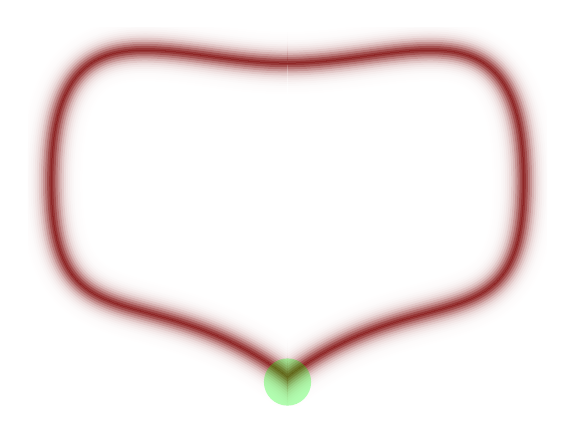
\begin{tikzpicture}[scale=0.3, thick]

\foreach \i in {0, 0.05,..., 1} {
  \begin{scope}
    \clip (-0.005, -9.5) rectangle (11, 6.5);
    \draw[line width={30 * \i}, opacity={exp(-8 * \i)}, dark] 
    (0, 5) .. controls (5, 5) and (10, 8) .. (10, 0)
             .. controls (10, -8) and (5, -3) .. (-2, -10);
  \end{scope}
  
  \begin{scope}
    \clip (0.005, -9.5) rectangle (-11, 6.5);
    \draw[line width={30 * \i}, opacity={exp(-8 * \i)}, dark] 
    (0, 5) .. controls (-5, 5) and (-10, 8) .. (-10, 0)
             .. controls (-10, -8) and (-5, -3) .. (2, -10);
  \end{scope}
}  
\fill[opacity=0.3, green] (0, -8.5) circle (1);
\end{tikzpicture}
%
\caption{Markov chains typically have trouble exploring regions 
of the typical set with large curvature (green), which induces
bias in Markov chain Monte Carlo estimators and spoils idealized
behavior such as Central Limit Theorems.}
\label{fig:pathological_typical_set}
\end{figure*}

Because Markov chains have to recover the exact expectations
asymptotically, they have to somehow compensate for not being
able to explore these regions.  Typically the Markov chain
accomplishes this by getting stuck near the boundary of the
pathological region: as it hovers the estimators are drawn down 
as if the Markov chain were exploring the pathological region.
Eventually the Markov chain escapes to explore the rest of the
typical set and the estimator bias begins to increase again
(Figure \ref{fig:pathological exploration}).  

\begin{figure*}
\centering
\subfigure[]{
\begin{tikzpicture}[scale=0.25, thick]
  \draw[-,color=white] (-12, 0) to (12, 0);
  
  \foreach \i in {0, 0.05,..., 1} {
    \begin{scope}
      \clip (-0.005, -9.5) rectangle (11, 6.5);
      \draw[line width={30 * \i}, opacity={exp(-8 * \i)}, dark] 
      (0, 5) .. controls (5, 5) and (10, 8) .. (10, 0)
               .. controls (10, -8) and (5, -3) .. (-2, -10);
    \end{scope}
  
    \begin{scope}
      \clip (0.005, -9.5) rectangle (-11, 6.5);
      \draw[line width={30 * \i}, opacity={exp(-8 * \i)}, dark] 
      (0, 5) .. controls (-5, 5) and (-10, 8) .. (-10, 0)
               .. controls (-10, -8) and (-5, -3) .. (2, -10);
    \end{scope}
  }  
  \fill[opacity=0.3, green] (0, -8.5) circle (1);
  
  \fill[color=dark] (-8, 5.5) circle (7pt);  
  \fill[color=light] (-8, 5.5) circle (5pt);  
  
  \fill[color=dark] (-9, 4.75) circle (7pt);  
  \fill[color=light] (-9, 4.75) circle (5pt);  

  \fill[color=dark] (-8.7, 4.6) circle (7pt);  
  \fill[color=light] (-8.7, 4.6) circle (5pt); 
  
  \fill[color=dark] (-9.1, 4.5) circle (7pt);  
  \fill[color=light] (-9.1, 4.5) circle (5pt);  
  
  \fill[color=dark] (-9.2, 3.5) circle (7pt);  
  \fill[color=light] (-9.2, 3.5) circle (5pt);   
  
  \fill[color=dark] (-9.9, 3) circle (7pt);  
  \fill[color=light] (-9.9, 3) circle (5pt); 
  
  \fill[color=dark] (-10.1, 2.15) circle (7pt);  
  \fill[color=light] (-10.1, 2.15) circle (5pt);   
  
  \fill[color=dark] (-9.6, 1.5) circle (7pt);  
  \fill[color=light] (-9.6, 1.5) circle (5pt);   
  
  \fill[color=dark] (-9.75, 1) circle (7pt);  
  \fill[color=light] (-9.75, 1) circle (5pt); 
  
  \fill[color=dark] (-10.2, 0.25) circle (7pt);  
  \fill[color=light] (-10.2, 0.25) circle (5pt); 
  
  \fill[color=dark] (-9.8, 0) circle (7pt);  
  \fill[color=light] (-9.8, 0) circle (5pt); 
  
  \fill[color=dark] (-10, -0.5) circle (7pt);  
  \fill[color=light] (-10, -0.5) circle (5pt); 
  
  \fill[color=dark] (-9.75, -2) circle (7pt);  
  \fill[color=light] (-9.75, -2) circle (5pt);
  
  \fill[color=dark] (-9.9, -3) circle (7pt);  
  \fill[color=light] (-9.9, -3) circle (5pt);  
  
  \fill[color=dark] (-9.25, -3.5) circle (7pt);  
  \fill[color=light] (-9.25, -3.5) circle (5pt);   
  
  \fill[color=dark] (-9, -4.25) circle (7pt);  
  \fill[color=light] (-9, -4.25) circle (5pt);   
     
  \fill[color=dark] (-8, -4.5) circle (7pt);  
  \fill[color=light] (-8, -4.5) circle (5pt);  
  
  \fill[color=dark] (-8.25, -4.75) circle (7pt);  
  \fill[color=light] (-8.25, -4.75) circle (5pt);  

  \fill[color=dark] (-7.75, -5) circle (7pt);  
  \fill[color=light] (-7.75, -5) circle (5pt);  
  
  \fill[color=dark] (-6.5, -5.5) circle (7pt);  
  \fill[color=light] (-6.5, -5.5) circle (5pt);  
  
  \fill[color=dark] (-5.75, -5.25) circle (7pt);  
  \fill[color=light] (-5.75, -5.25) circle (5pt);  
  
  \fill[color=dark] (-5, -6) circle (7pt);  
  \fill[color=light] (-5, -6) circle (5pt);  
  
  \fill[color=dark] (-4.75, -6.25) circle (7pt);  
  \fill[color=light] (-4.75, -6.25) circle (5pt);  
  
  \fill[color=dark] (-3.8, -6) circle (7pt);  
  \fill[color=light] (-3.8, -6) circle (5pt);  
  
  \fill[color=dark] (-3.25, -6.5) circle (7pt);  
  \fill[color=light] (-3.25, -6.5) circle (5pt); 
  
  \fill[color=dark] (-2.75, -6.75) circle (7pt);  
  \fill[color=light] (-2.75, -6.75) circle (5pt);   
  
  \fill[color=dark] (-2, -7.5) circle (7pt);  
  \fill[color=light] (-2, -7.5) circle (5pt); 
  
  \fill[color=dark] (-1.75, -6.8) circle (7pt);  
  \fill[color=light] (-1.75, -6.8) circle (5pt);  
  
  \fill[color=dark] (-1.5, -7.2) circle (7pt);  
  \fill[color=light] (-1.5, -7.2) circle (5pt); 

  \draw[-,color=white] (14, 0) to (38, 0);  
  \node[] at (28,-2) {\includegraphics[width=6cm]{funnel_trace1.eps}};
\end{tikzpicture}
}
\subfigure[]{
\begin{tikzpicture}[scale=0.25, thick]
  \draw[-,color=white] (-12, 0) to (12, 0);
  
  \foreach \i in {0, 0.05,..., 1} {
    \begin{scope}
      \clip (-0.005, -9.5) rectangle (11, 6.5);
      \draw[line width={30 * \i}, opacity={exp(-8 * \i)}, dark] 
      (0, 5) .. controls (5, 5) and (10, 8) .. (10, 0)
               .. controls (10, -8) and (5, -3) .. (-2, -10);
    \end{scope}
  
    \begin{scope}
      \clip (0.005, -9.5) rectangle (-11, 6.5);
      \draw[line width={30 * \i}, opacity={exp(-8 * \i)}, dark] 
      (0, 5) .. controls (-5, 5) and (-10, 8) .. (-10, 0)
               .. controls (-10, -8) and (-5, -3) .. (2, -10);
    \end{scope}
  }  
  \fill[opacity=0.3, green] (0, -8.5) circle (1);
  
  \fill[color=dark] (-8, 5.5) circle (7pt);  
  \fill[color=light] (-8, 5.5) circle (5pt);  
  
  \fill[color=dark] (-9, 4.75) circle (7pt);  
  \fill[color=light] (-9, 4.75) circle (5pt);  

  \fill[color=dark] (-8.7, 4.6) circle (7pt);  
  \fill[color=light] (-8.7, 4.6) circle (5pt); 
  
  \fill[color=dark] (-9.1, 4.5) circle (7pt);  
  \fill[color=light] (-9.1, 4.5) circle (5pt);  
  
  \fill[color=dark] (-9.2, 3.5) circle (7pt);  
  \fill[color=light] (-9.2, 3.5) circle (5pt);   
  
  \fill[color=dark] (-9.9, 3) circle (7pt);  
  \fill[color=light] (-9.9, 3) circle (5pt); 
  
  \fill[color=dark] (-10.1, 2.15) circle (7pt);  
  \fill[color=light] (-10.1, 2.15) circle (5pt);   
  
  \fill[color=dark] (-9.6, 1.5) circle (7pt);  
  \fill[color=light] (-9.6, 1.5) circle (5pt);   
  
  \fill[color=dark] (-9.75, 1) circle (7pt);  
  \fill[color=light] (-9.75, 1) circle (5pt); 
  
  \fill[color=dark] (-10.2, 0.25) circle (7pt);  
  \fill[color=light] (-10.2, 0.25) circle (5pt); 
  
  \fill[color=dark] (-9.8, 0) circle (7pt);  
  \fill[color=light] (-9.8, 0) circle (5pt); 
  
  \fill[color=dark] (-10, -0.5) circle (7pt);  
  \fill[color=light] (-10, -0.5) circle (5pt); 
  
  \fill[color=dark] (-9.75, -2) circle (7pt);  
  \fill[color=light] (-9.75, -2) circle (5pt);
  
  \fill[color=dark] (-9.9, -3) circle (7pt);  
  \fill[color=light] (-9.9, -3) circle (5pt);  
  
  \fill[color=dark] (-9.25, -3.5) circle (7pt);  
  \fill[color=light] (-9.25, -3.5) circle (5pt);   
  
  \fill[color=dark] (-9, -4.25) circle (7pt);  
  \fill[color=light] (-9, -4.25) circle (5pt);   
     
  \fill[color=dark] (-8, -4.5) circle (7pt);  
  \fill[color=light] (-8, -4.5) circle (5pt);  
  
  \fill[color=dark] (-8.25, -4.75) circle (7pt);  
  \fill[color=light] (-8.25, -4.75) circle (5pt);  

  \fill[color=dark] (-7.75, -5) circle (7pt);  
  \fill[color=light] (-7.75, -5) circle (5pt);  
  
  \fill[color=dark] (-6.5, -5.5) circle (7pt);  
  \fill[color=light] (-6.5, -5.5) circle (5pt);  
  
  \fill[color=dark] (-5.75, -5.25) circle (7pt);  
  \fill[color=light] (-5.75, -5.25) circle (5pt);  
  
  \fill[color=dark] (-5, -6) circle (7pt);  
  \fill[color=light] (-5, -6) circle (5pt);  
  
  \fill[color=dark] (-4.75, -6.25) circle (7pt);  
  \fill[color=light] (-4.75, -6.25) circle (5pt);  
  
  \fill[color=dark] (-3.8, -6) circle (7pt);  
  \fill[color=light] (-3.8, -6) circle (5pt);  
  
  \fill[color=dark] (-3.25, -6.5) circle (7pt);  
  \fill[color=light] (-3.25, -6.5) circle (5pt); 
  
  \fill[color=dark] (-2.75, -6.75) circle (7pt);  
  \fill[color=light] (-2.75, -6.75) circle (5pt);   
  
  \fill[color=dark] (-2, -7.5) circle (7pt);  
  \fill[color=light] (-2, -7.5) circle (5pt); 
  
  \fill[color=dark] (-1.75, -6.8) circle (7pt);  
  \fill[color=light] (-1.75, -6.8) circle (5pt);  
  
  \fill[color=dark] (-1.5, -7.2) circle (7pt);  
  \fill[color=light] (-1.5, -7.2) circle (5pt); 
  
  \fill[color=dark] (-0.5, -7.5) circle (7pt);  
  \fill[color=light] (-0.5, -7.5) circle (5pt);
  
  \fill[color=dark] (0, -7.6) circle (7pt);  
  \fill[color=light] (0, -7.6) circle (5pt);  
  
  \fill[color=dark] (1, -7.7) circle (7pt);  
  \fill[color=light] (1, -7.7) circle (5pt);  

  \draw[-,color=white] (14, 0) to (38, 0);  
  \node[] at (28,-2) {\includegraphics[width=6cm]{funnel_trace2.eps}};
\end{tikzpicture}
}
\subfigure[]{
\begin{tikzpicture}[scale=0.25, thick]
  \draw[-,color=white] (-12, 0) to (12, 0);
  
  \foreach \i in {0, 0.05,..., 1} {
    \begin{scope}
      \clip (-0.005, -9.5) rectangle (11, 6.5);
      \draw[line width={30 * \i}, opacity={exp(-8 * \i)}, dark] 
      (0, 5) .. controls (5, 5) and (10, 8) .. (10, 0)
               .. controls (10, -8) and (5, -3) .. (-2, -10);
    \end{scope}
  
    \begin{scope}
      \clip (0.005, -9.5) rectangle (-11, 6.5);
      \draw[line width={30 * \i}, opacity={exp(-8 * \i)}, dark] 
      (0, 5) .. controls (-5, 5) and (-10, 8) .. (-10, 0)
               .. controls (-10, -8) and (-5, -3) .. (2, -10);
    \end{scope}
  }  
  \fill[opacity=0.3, green] (0, -8.5) circle (1);
  
  \fill[color=dark] (-8, 5.5) circle (7pt);  
  \fill[color=light] (-8, 5.5) circle (5pt);  
  
  \fill[color=dark] (-9, 4.75) circle (7pt);  
  \fill[color=light] (-9, 4.75) circle (5pt);  

  \fill[color=dark] (-8.7, 4.6) circle (7pt);  
  \fill[color=light] (-8.7, 4.6) circle (5pt); 
  
  \fill[color=dark] (-9.1, 4.5) circle (7pt);  
  \fill[color=light] (-9.1, 4.5) circle (5pt);  
  
  \fill[color=dark] (-9.2, 3.5) circle (7pt);  
  \fill[color=light] (-9.2, 3.5) circle (5pt);   
  
  \fill[color=dark] (-9.9, 3) circle (7pt);  
  \fill[color=light] (-9.9, 3) circle (5pt); 
  
  \fill[color=dark] (-10.1, 2.15) circle (7pt);  
  \fill[color=light] (-10.1, 2.15) circle (5pt);   
  
  \fill[color=dark] (-9.6, 1.5) circle (7pt);  
  \fill[color=light] (-9.6, 1.5) circle (5pt);   
  
  \fill[color=dark] (-9.75, 1) circle (7pt);  
  \fill[color=light] (-9.75, 1) circle (5pt); 
  
  \fill[color=dark] (-10.2, 0.25) circle (7pt);  
  \fill[color=light] (-10.2, 0.25) circle (5pt); 
  
  \fill[color=dark] (-9.8, 0) circle (7pt);  
  \fill[color=light] (-9.8, 0) circle (5pt); 
  
  \fill[color=dark] (-10, -0.5) circle (7pt);  
  \fill[color=light] (-10, -0.5) circle (5pt); 
  
  \fill[color=dark] (-9.75, -2) circle (7pt);  
  \fill[color=light] (-9.75, -2) circle (5pt);
  
  \fill[color=dark] (-9.9, -3) circle (7pt);  
  \fill[color=light] (-9.9, -3) circle (5pt);  
  
  \fill[color=dark] (-9.25, -3.5) circle (7pt);  
  \fill[color=light] (-9.25, -3.5) circle (5pt);   
  
  \fill[color=dark] (-9, -4.25) circle (7pt);  
  \fill[color=light] (-9, -4.25) circle (5pt);   
     
  \fill[color=dark] (-8, -4.5) circle (7pt);  
  \fill[color=light] (-8, -4.5) circle (5pt);  
  
  \fill[color=dark] (-8.25, -4.75) circle (7pt);  
  \fill[color=light] (-8.25, -4.75) circle (5pt);  

  \fill[color=dark] (-7.75, -5) circle (7pt);  
  \fill[color=light] (-7.75, -5) circle (5pt);  
  
  \fill[color=dark] (-6.5, -5.5) circle (7pt);  
  \fill[color=light] (-6.5, -5.5) circle (5pt);  
  
  \fill[color=dark] (-5.75, -5.25) circle (7pt);  
  \fill[color=light] (-5.75, -5.25) circle (5pt);  
  
  \fill[color=dark] (-5, -6) circle (7pt);  
  \fill[color=light] (-5, -6) circle (5pt);  
  
  \fill[color=dark] (-4.75, -6.25) circle (7pt);  
  \fill[color=light] (-4.75, -6.25) circle (5pt);  
  
  \fill[color=dark] (-3.8, -6) circle (7pt);  
  \fill[color=light] (-3.8, -6) circle (5pt);  
  
  \fill[color=dark] (-3.25, -6.5) circle (7pt);  
  \fill[color=light] (-3.25, -6.5) circle (5pt); 
  
  \fill[color=dark] (-2.75, -6.75) circle (7pt);  
  \fill[color=light] (-2.75, -6.75) circle (5pt);   
  
  \fill[color=dark] (-2, -7.5) circle (7pt);  
  \fill[color=light] (-2, -7.5) circle (5pt); 
  
  \fill[color=dark] (-1.75, -6.8) circle (7pt);  
  \fill[color=light] (-1.75, -6.8) circle (5pt);  
  
  \fill[color=dark] (-1.5, -7.2) circle (7pt);  
  \fill[color=light] (-1.5, -7.2) circle (5pt); 
    
  \fill[color=dark] (-0.5, -7.5) circle (7pt);  
  \fill[color=light] (-0.5, -7.5) circle (5pt);
  
  \fill[color=dark] (0, -7.6) circle (7pt);  
  \fill[color=light] (0, -7.6) circle (5pt);  
  
  \fill[color=dark] (1, -7.7) circle (7pt);  
  \fill[color=light] (1, -7.7) circle (5pt);  
  
  \fill[color=dark] (9, 4.7) circle (7pt);  
  \fill[color=light] (9, 4.7) circle (5pt);  
  
  \fill[color=dark] (9.1, 4.25) circle (7pt);  
  \fill[color=light] (9.1, 4.25) circle (5pt);   
  
  \fill[color=dark] (9.8, 3) circle (7pt);  
  \fill[color=light] (9.8, 3) circle (5pt);   
  
  \fill[color=dark] (9.9, 1.5) circle (7pt);  
  \fill[color=light] (9.9, 1.5) circle (5pt);   
  
  \fill[color=dark] (9.75, -0.5) circle (7pt);  
  \fill[color=light] (9.75, -0.5) circle (5pt); 
  
  \fill[color=dark] (9.9, -1) circle (7pt);  
  \fill[color=light] (9.9, -1) circle (5pt);
  
  \fill[color=dark] (9.6, -3.5) circle (7pt);  
  \fill[color=light] (9.6, -3.5) circle (5pt);   
     
  \fill[color=dark] (7.8, -4.5) circle (7pt);  
  \fill[color=light] (7.8, -4.5) circle (5pt);  
  
  \fill[color=dark] (7, -5) circle (7pt);  
  \fill[color=light] (7, -5) circle (5pt);  
  
  \fill[color=dark] (6.5, -5.5) circle (7pt);  
  \fill[color=light] (6.5, -5.5) circle (5pt);  
  
  \fill[color=dark] (4.25, -6.5) circle (7pt);  
  \fill[color=light] (4.25, -6.5) circle (5pt);  
  
  \fill[color=dark] (2.1, -6.5) circle (7pt);  
  \fill[color=light] (2.1, -6.5) circle (5pt);   
  
  \draw[-,color=white] (14, 0) to (38, 0);  
  \node[] at (28,-2) {\includegraphics[width=6cm]{funnel_trace3.eps}};
\end{tikzpicture}
}
\caption{In practice, pathological regions of the typical set usually
cause Markov chains to get ``stuck''.  (a) Initial the Markov chain 
explores well-behaved regions of the typical set, avoiding the 
pathological neighborhood entirely and biasing Markov chain
Monte Carlo estimators.  (b) If the Markov chain is run long enough
then it will get stuck near the boundary of the pathological region, 
slowly correcting the Markov chain Monte Carlo estimators.  (c) 
Eventually the Markov chain escapes and explores the rest of 
the typical set.  This process repeats causing the resulting 
estimators to oscillate around the true expectations in an unstable 
fashion.}
\label{fig:pathological exploration}
\end{figure*}

Ultimately this behavior results in estimators that oscillate 
around the true expectations.  Asymptotically the oscillations
average out the true values, but that balance is delicate and
any finite time estimator will suffer from substantial biases.

Whether or not features of the target distribution become
pathological depends on how the Markov transition kernel
interacts with the target distribution.  Some transition kernels
are more robust than others and some can achieve robust
performance with careful tuning of auxiliary kernel parameters.
 
\subsubsection{MCMC in Practice}

In order to guarantee that we will not suffer from pathological
behavior we have to demonstrate strong \emph{ergodicity}
conditions that ensure the Markov chain not only explores
the typical set but does so sufficiently fast.  In most cases
we need to establish \emph{geometric ergodicity}.

Although we can identify generic features that often prevent
geometric ergodicity, determining whether or not a particular
Markov chain will exhibit pathological behavior when 
targeting a particular distribution is almost always infeasible
for nontrivial problems.  Moreover, there are no sufficient
conditions that we can use to establish geometric ergodicity
empirically.  Instead we have to rely on necessary conditions 
to provide evidence that we can trust the resulting Markov 
chain Monte Carlo estimators.

Consequently we have to take great care when implementing
Markov chain Monte Carlo.  We proceed in three stages.

\vspace{2mm}
\noindent \emph{Warmup}
\vspace{2mm}

We begin with \emph{warmup}, where we initialize multiple
chains from multiple, ideally diffuse, points in the sample space
and run long enough for them to converge to the typical set.
Because we do not include these warmup samples in any
Markov chain Monte Carlo estimators, we can also use this
period to adaptively tune any parameters in the Markov 
kernel without biasing our estimates.

Historically this stage has usually been called \emph{burn-in},
but we find that terminology inappropriate for Markov chain
Monte Carlo.  The problem is that burn-in is a process of 
stress-testing a system to identify and replace any failing
components.  In Markov chain Monte Carlo, however, any
misbehaving chains identify pathological behavior that is
biasing all of the chains and should very much not be ignored.
Because of this potentially-confusing false analogy we use the
term warmup.

\vspace{2mm}
\noindent \emph{Sampling}
\vspace{2mm}

Once warmup as finished we begin a sampling phase where
we run the Markov chain and save all of the resulting samples
to construct Markov chain Monte Carlo estimators.

\vspace{2mm}
\noindent \emph{Evaluation}
\vspace{2mm}

Once both warmup and sampling have completed we can
search for any signs of pathological behavior and, if we
can't find any, move on to computing any desired estimator.

For what kind of pathological behavior should we be looking?
Well if we don't run warmup long enough for all of the Markov
chains to converge then not all of the Markov chains will look 
the same.  Similarly, any pathological regions in the typical set 
will bias the Markov chains in different ways.  Consequently a 
necessary condition for robust Markov chain Monte Carlo 
estimators is that each Markov chain appears identical.  In theory
we can quantify the homogeneity of our ensemble of Markov chains 
with the \emph{potential scale reduction factor} and in practice we
can estimate the potential scale reduction factor with the $\hat{R}$
statistic.

In addition to $\hat{R}$, specific Markov transitions may admit
their own, unique diagnostics sensitive to various pathologies
that can frustrate geometric ergodicity.

If we are confident that our Markov chains are exploring without
obstruction then we can finally compute Markov chain Monte
Carlo estimators using the samples generated in the sampling
phase.  If we also estimate the variances and autocorrelations
of each function then we can also quantify the error of these
estimates using an estimate of the Markov chain Monte Carlo
Standard Error.

\section{Bayesian Inference}

With a foundation of probability theory we are now ready to
formally define concepts like measurement, inference, and 
decision making.  Here we consider a Bayesian approach
to these ideas, although the same foundation is also critical
for constructing a frequentist approach.

We begin by defining measurements and what we want
to learn from those measurements, and then consider how
we approximate that system in practice with an abstract
mathematical model.  Once we have defined a model we
can define how we learn from that model and then how
we make decisions with that model.

\subsection{Measurements}

The basic assumption underlying inference is that there is some
observable process that we would like to understand, or at least
some latent process that has observable consequences.

These observable consequences manifest as logical statements,
but in practice we can observe only variable measurements
of those statements.  In order to formalize these concepts we
assume that this variability is sufficiently well-behaved that we
can describe it with probability theory.  More formally, we assume
that the process under consideration defines a probability 
distribution, $\PP_{D}$ over some measurement space, $D$, 
with measurements defined as events in the corresponding
event space.  

Although we have assumed the existence of a \emph{data
generating process}, $\PP_{D}$, we have intentionally not
assumed any philosophical interpretation of it.  In particular, we
are indifferent to the ultimate source of the variability in the
measurements quantified by $\PP_{D}$: it could be some
ontological variability inherent to the system or just some
epistemological variability due to our ignorance of the underlying 
system.  The only assumption we have made is that the
measurements are repeatable and variable, and that this
variability is sufficiently well-behaved to be described by a 
mathematical model. 

Although we can assume the existence of a data generating 
process, we don't know anything about it until we start making 
measurements.  An infinite number of measurements would 
certainly inform us of the data generating process exactly,
but measurements are expensive and in practice we have
to learn about the data generating process from only a few
measurements, if not just a single measurements. \emph{Inference}
is the process of learning about the data generating process
using only a finite number measurements.  

\subsection{Big Worlds and Small Worlds}

If we want to learn about the data generating process we have
to consider all possible data generating process we could
encounter or, equivalently, all possible probability distributions
over the sample space, $D$.  We refer to this massive set, $\mathcal{P}_{D}$
as the \emph{the big world} (Figure \ref{fig:big_world}).  

\begin{figure*}
\centering
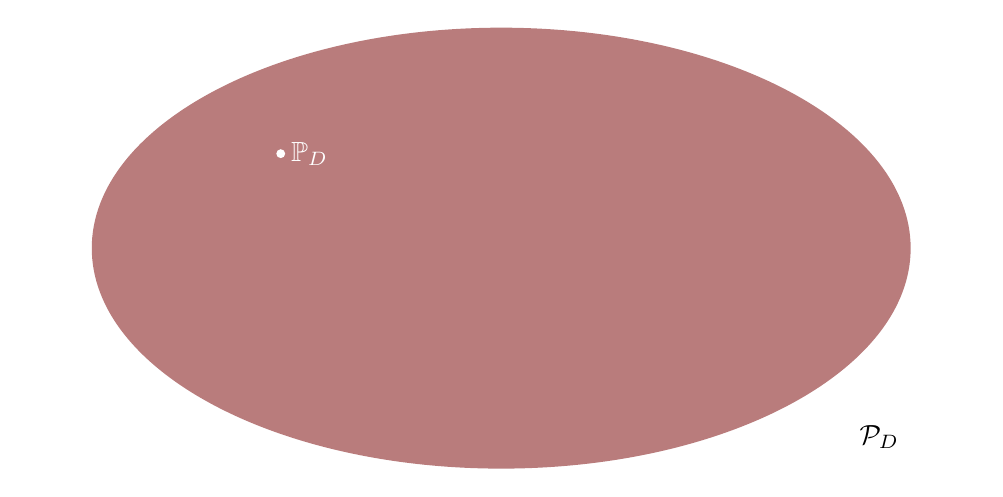
\begin{tikzpicture}[scale=0.40, thick]

  \draw[color=white] (-15, 0) -- (15, 0);

  \fill[mid] (0, 0) ellipse (13 and 7);
  \node at (12, -6) {$\mathcal{P}_{D}$};
  
  \fill[color=white] (-7, 3) circle (4pt)
  node[right, color=white] {$\PP_{D}$};
  
\end{tikzpicture}
\caption{Once we have defined a measurement space, $D$, the latent data
generating process, $\PP_{D}$ can be found in the space of all possible
data generating processes over $D$, $\mathcal{P}_{D}$.
}
\label{fig:big_world}
\end{figure*}

The big world is much to ungainly to be even be well-defined in practice, 
let alone exhaustively explored.  Instead we have to limit our consideration 
to only a subset of probability distributions over the measurement space 
called a \emph{small world}, $\Theta \subset \mathcal{P}_{D}$ 
(Figure \ref{fig:small_worlds}a).

Each point in the small world, $\theta \in \Theta$, identifies a unique 
probability distribution over data.  Consequently the small world is 
equivalent to a probability distribution over the measurements space
conditioned on the small world,
%
\begin{align*}
\mathbb{L}
&: \EV{D} \times \Theta \rightarrow \left[0, 1 \right] \\
&\quad \left( E_{D}, \theta \right) \;\; \mapsto 
\mathbb{L} \! \left[ E_{D} \mid \theta \right].
\end{align*}
%
This conditional probability distribution is also known as the 
\emph{likelihood}.

Regardless of how it is chosen, the assumption of any specific 
small world can have drastic limitations on inference.  Because any
small world is likely to be only a shallow approximation of reality,
for example, it is probability to contain the latent data generating
process (Figure \ref{fig:small_worlds}b).  Consequently even ideal
inferences are subject to error, and the utility of any inference
always depends on the viability of our assumptions.

\begin{figure*}
\centering
%
\subfigure[]{
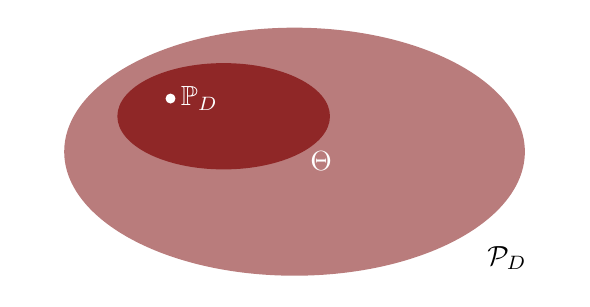
\begin{tikzpicture}[scale=0.225, thick]
  
  \draw[color=white] (-15, 0) -- (15, 0);
  
  \fill[mid] (0, 0) ellipse (13 and 7);
  \node at (12, -6) {$\mathcal{P}_{D}$};
  
  \fill[dark] (-4, 2) ellipse (6 and 3);
  \node[color=white] at (1.5, -0.5) {$\Theta$};
  
  \fill[color=white] (-7, 3) circle (8pt)
  node[right, color=white] {$\PP_{D}$};
  
\end{tikzpicture}
}
\subfigure[]{
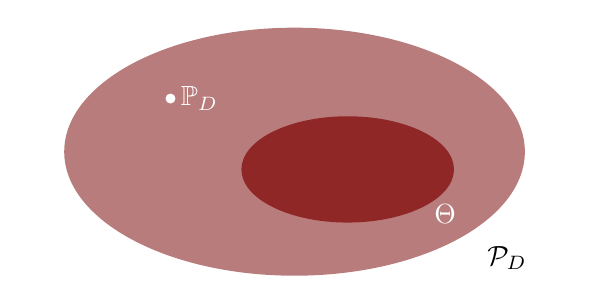
\begin{tikzpicture}[scale=0.225, thick]

  \draw[color=white] (-15, 0) -- (15, 0);

  \fill[mid] (0, 0) ellipse (13 and 7);
  \node at (12, -6) {$\mathcal{P}_{D}$};
  
  \fill[dark] (3, -1) ellipse (6 and 3);
  \node[color=white] at (8.5, -3.5) {$\Theta$};
  
  \fill[color=white] (-7, 3) circle (8pt)
  node[right, color=white] {$\PP_{D}$};
  
\end{tikzpicture}
}
\caption{Practical inference requires the selection of a distinguished subset 
of data generating processes called a small world, $\Theta$, that (a) may or 
(b) may not contain the latent data generating process, $\PP_{D}$.  The 
Boxian philosophy of ``all models are wrong but some are useful'' asserts 
that the former is impossible in practical problems, but even in the latter
the probability distributions in the small world may provide useful approximations 
of $\PP_{D}$.
}
\label{fig:small_worlds}
\end{figure*}

\subsection{Uncertainty And Learning In The Small World}

We have already used probability theory to quantify the variability of measurements,
but now we can also use probability theory to quantify our uncertainty about which
elements of the small world are good approximations to the latent data
generating process.  

The \emph{prior distribution}, $\PP_{\Theta}^{\mathrm{prior}}$, is a probability 
distribution over the small world that quantifies our initial uncertainty about 
which elements are most consistent with the latent data generating process.  
The information inherent in the prior distribution can come from previous 
measurements, theoretical constraints, or even elicitation of experts.  

Learning in the small world is the process of the updating of the prior distribution
with any information contained in the measurement to give a \emph{posterior
distribution}, $\PP_{\Theta}^{\mathrm{post}}$, that quantifies our uncertainty
about the small world after the measurement  (Figure \ref{fig:learning}).  The 
likelihood implicit defines any information contained in a measurement and 
then the actual mechanism for this update is immediately given by probability 
theory.  It is most simply written in terms of probability density functions,
%
\begin{equation*}
p^{\mathrm{post}} \! \left( \theta \mid d \right)
\propto
L \! \left( d \mid \theta \right) p^{\mathrm{prior}} \! \left( \theta \right),
\end{equation*}
%
which can be recognized as the celebrated Bayes' Theorem.

Bayes' Theorem, however, is just a mathematical consequence of probability
theory and its appearance is an inevitability once we use probabilities to
quantify our uncertainty about the small world.  Ultimately, all of this
abstraction is just means to formalize the intuition that \emph{what we know 
after a measurement is what we knew before the measurement plus any 
information contained in the measurement}.

\begin{figure*}
\centering
%
\subfigure[]{
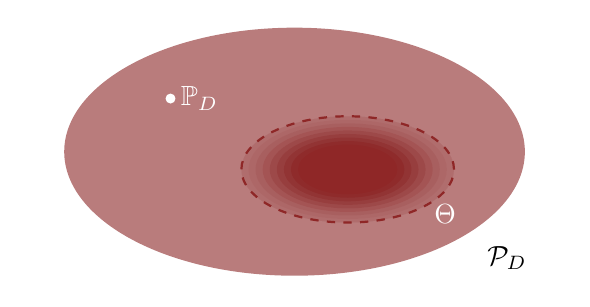
\begin{tikzpicture}[scale=0.225, thick]

  \draw[color=white] (-15, 0) -- (15, 0);

  \fill[mid] (0, 0) ellipse (13 and 7);
  \node at (12, -6) {$\mathcal{P}_{D}$};
  
  \draw[color=dark, dashed] (3, -1) ellipse (6 and 3);
  \node[color=white] at (8.5, -3.5) {$\Theta$};
  
  \fill[color=white] (-7, 3) circle (8pt)
  node[right, color=white] {$\PP_{D}$};
  
  \begin{scope}
    \clip (3, -1) ellipse (6 and 3);
    \foreach \i in {0, 0.05,..., 1} {
      \fill[opacity={exp(-5 * \i*\i)}, dark] (3, -1) ellipse ({8 * \i} and {4 * \i});      
    }
  \end{scope}
  
\end{tikzpicture}
}
%
\subfigure[]{
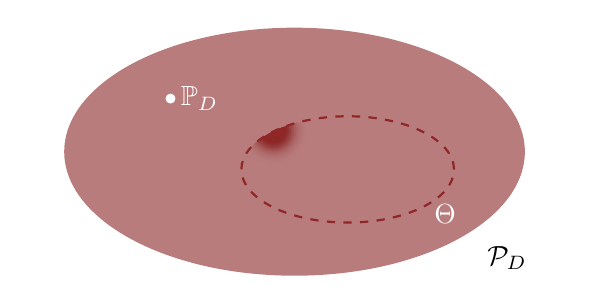
\begin{tikzpicture}[scale=0.225, thick]

  \draw[color=white] (-15, 0) -- (15, 0);

  \fill[mid] (0, 0) ellipse (13 and 7);
  \node at (12, -6) {$\mathcal{P}_{D}$};
  
  \draw[color=dark, dashed] (3, -1) ellipse (6 and 3);
  \node[color=white] at (8.5, -3.5) {$\Theta$};
  
  \fill[color=white] (-7, 3) circle (8pt)
  node[right, color=white] {$\PP_{D}$};
  
  \begin{scope}
    \clip (3, -1) ellipse (6 and 3);
    \foreach \i in {0, 0.05,..., 1} {
      \fill[opacity={exp(-5 * \i*\i)}, dark] (-1.2, 1.2) circle ({2 * \i});      
    }
  \end{scope}
  
\end{tikzpicture}
}
\caption{Inference in the small world is the process of updating
(a) a prior distribution quantifying our initial uncertainty about the small
world into (b) a posterior distribution quantifying our uncertainty about
the small world after incorporating any information in a measurement.
If all of our assumptions are viable then the posterior should concentrate
towards the latent data generating process, $\PP_{D}$.
}
\label{fig:learning}
\end{figure*}

\subsection{TODO: Decision Making in the Small World}

Now that we've quantified uncertainty we can make robust decisions.

Formalize with a risk/utility function, compute expected risk/utility, then
chose the decision that minimizes/maximizes the expected risk/utility.

\subsection{TODO: Bayesian Inference in Practice}

Model a prior and a likelihood.  Posterior is immediately given and
all statements about our system, including decisions, are given by
expectations.  As discussed above we have many options for
approximating those expectations in practice.

The biggest challenge in implementing Bayesian inference, then,
is the actual modeling of the prior and likelihood.  Much can be
said about both, but let's take a second to discuss one of the most
powerful means of methods of building small worlds: \emph{generative modeling}.  
Here we build up the small world
sequentially by modeling each state of the data generating process.
For example, we might build a small world for polling data by
modeling the sampling of an individual from a population and
then a series of non-responses based on the individual's demographics.
Or we might have a strong physical model, which we can wrap
in an equality complex measurement model to account for the
various systematic effects introduced in the measurement process.
Any such model will be an approximation to the true generative
process, but this perspective allows us to build better and better
approximations by adding more and more detail as necessary.
\textbf{Natural way to unite user intuition with explicit modeling.}
\textbf{More detail in examples, emphasizing modeling of
measurement process.}

\textbf{Generative models as a way to define small worlds with
disintegrations.  Does not necessarily imply causal structure
but the more casual structure the better!}

\subsection{TODO: Checking Model Assumptions with Predictive Performance}

Checking model assumptions with posterior predictive checks.

\begin{figure*}
\centering
%
\subfigure[]{
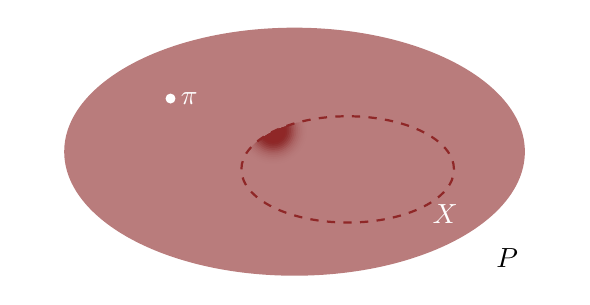
\begin{tikzpicture}[scale=0.225, thick]
  \draw[color=white] (-15, 0) -- (15, 0);

  \fill[mid] (0, 0) ellipse (13 and 7);
  \node at (12, -6) {$P$};
  
  \draw[color=dark, dashed] (3, -1) ellipse (6 and 3);
  \node[color=white] at (8.5, -3.5) {$X$};
  
  \fill[color=white] (-7, 3) circle (8pt)
  node[right, color=white] {$\pi$};
  
  \begin{scope}
    \clip (3, -1) ellipse (6 and 3);
    \foreach \i in {0, 0.05,..., 1} {
      \fill[opacity={exp(-5 * \i*\i)}, dark] (-1.2, 1.2) circle ({2 * \i});      
    }
  \end{scope} 
\end{tikzpicture}
}
%
\subfigure[]{
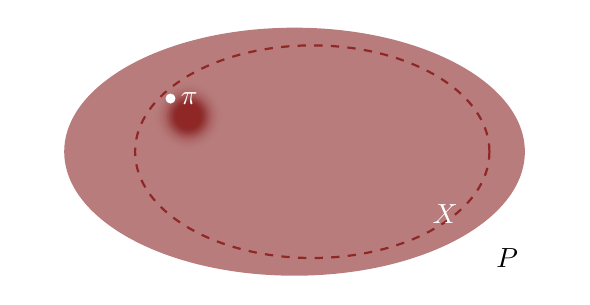
\begin{tikzpicture}[scale=0.225, thick]
  \draw[color=white] (-15, 0) -- (15, 0);

  \fill[mid] (0, 0) ellipse (13 and 7);
  \node at (12, -6) {$P$};
  
  \draw[color=dark, dashed] (1, 0) ellipse (10 and 6);
  \node[color=white] at (8.5, -3.5) {$X$};
  
   \begin{scope}
    \clip (1, 0) ellipse (10 and 6);
    \foreach \i in {0, 0.05,..., 1} {
      \fill[opacity={exp(-5 * \i*\i)}, dark] (-6, 2) circle ({2 * \i});      
    }
  \end{scope}
  
  \fill[color=white] (-7, 3) circle (8pt)
  node[right, color=white] {$\pi$};
\end{tikzpicture}
}
\caption{Cartoon of model updating.
}
\label{fig:model_updating}
\end{figure*}

\end{document}  